\section{Numerical Experiments}\label{s-experiments}

\begin{figure}
	\centering
	\begin{subfigure}{0.3\textwidth}
		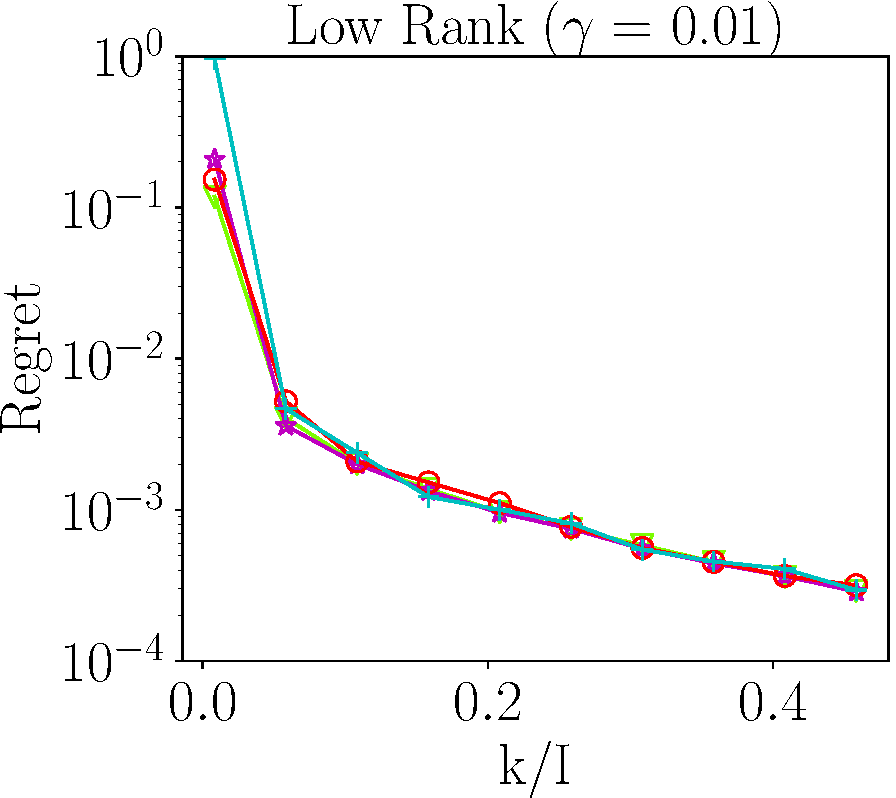
\includegraphics[scale = 0.24]{figure/fig2_lk_lnoise_600.pdf}
	\end{subfigure}
	\begin{subfigure}{0.3\textwidth}
		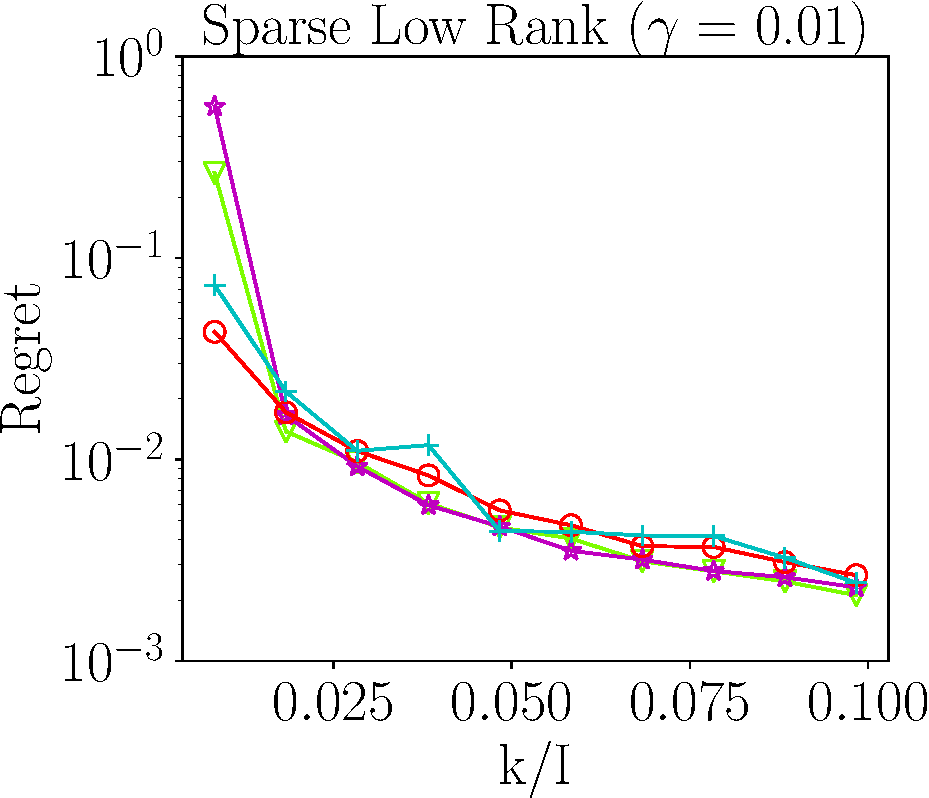
\includegraphics[scale = 0.24]{figure/fig2_slk_lnoise_600.pdf}
	\end{subfigure}
	\begin{subfigure}{0.3\textwidth}
		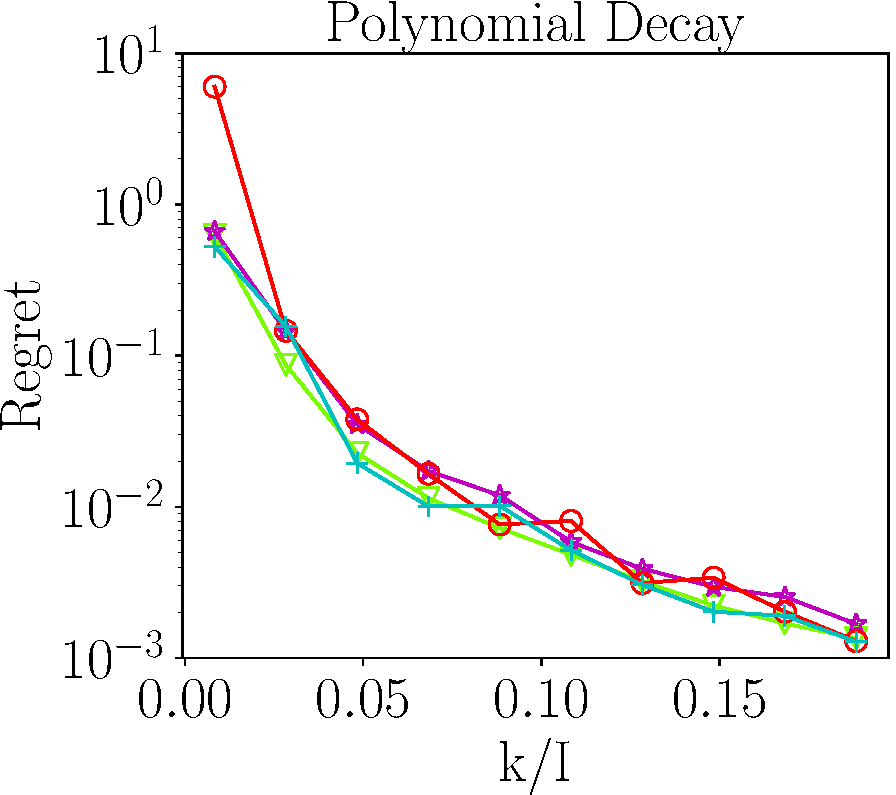
\includegraphics[scale = 0.24]{figure/fig2_spd_600.pdf}
	\end{subfigure}\\
	\begin{subfigure}{0.3\textwidth}
		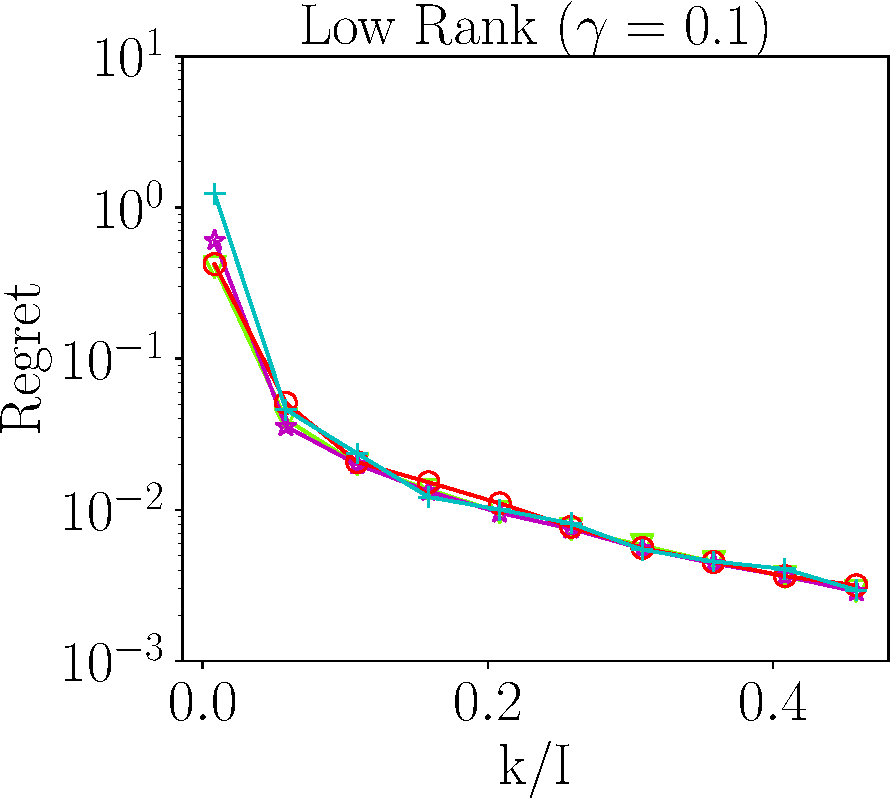
\includegraphics[scale = 0.24]{figure/fig2_lk_mnoise_600.pdf}
	\end{subfigure}
	\begin{subfigure}{0.5\textwidth}
		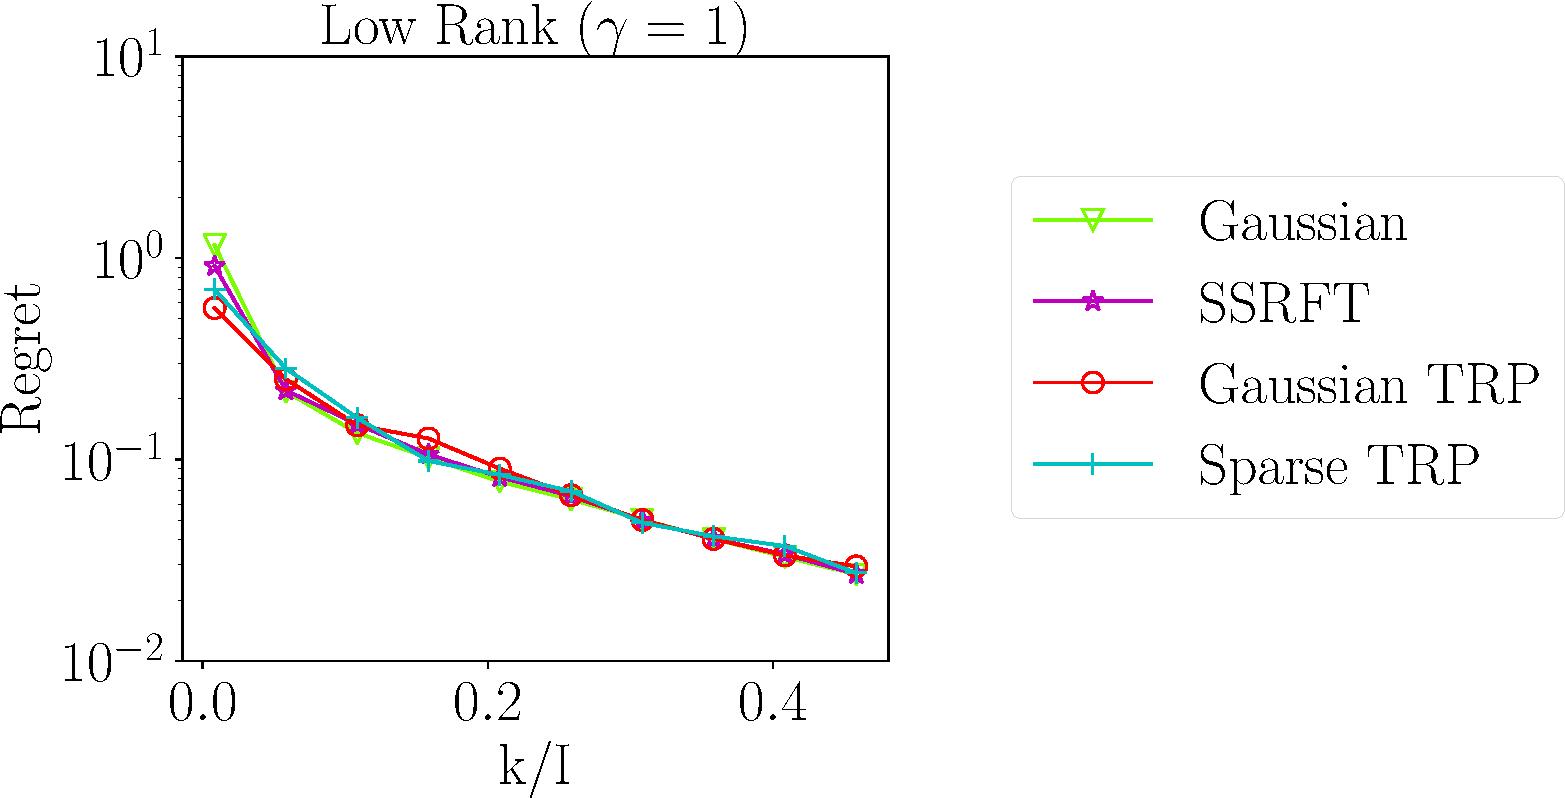
\includegraphics[scale = 0.24]{figure/fig2_lk_hnoise_600.pdf}
	\end{subfigure}
	\\
	\caption{\textit{Different DRMs perform similarly.}
		We approximate 3D synthetic tensors (see \ref{s-synthetic-data}) with $I = 600$,
		using our one-pass algorithm with $r = 5$ and varying $k$ ($s = 2k+1$),
		using a variety of DRMs in the Tucker sketch:
		Gaussian, SSRFT, Gaussian TRP, or Sparse TRP.
		\label{fig:vary-k-600}
	}
\end{figure}

\begin{figure}
	\centering
	\begin{subfigure}{0.3\textwidth}
		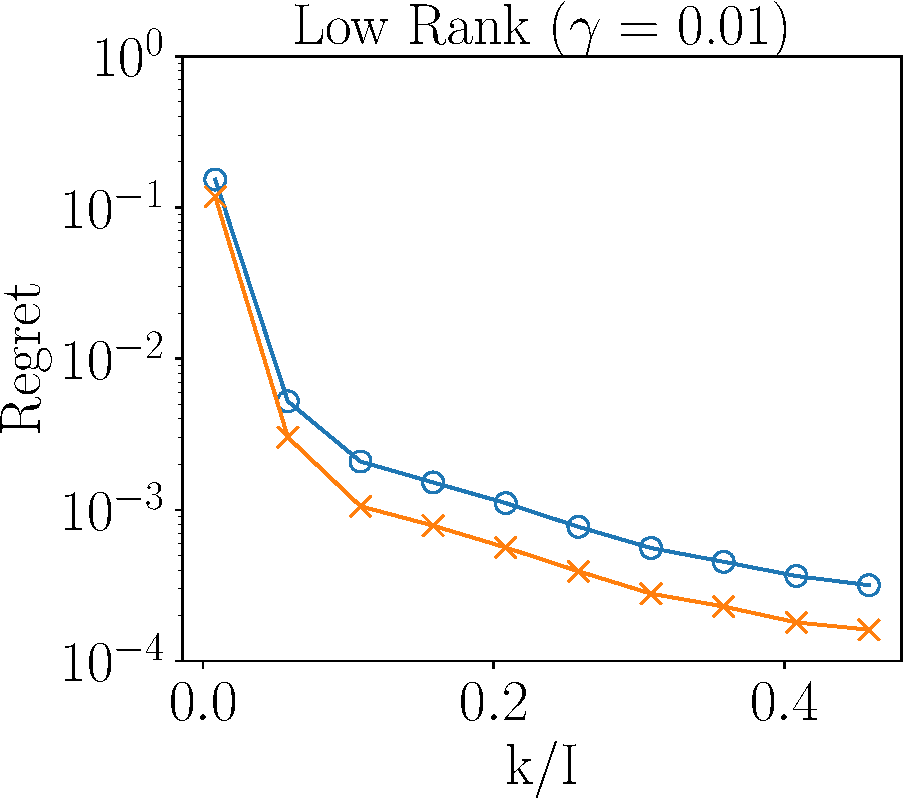
\includegraphics[scale = 0.24]{figure/fig3_lk_lnoise_600.pdf}
	\end{subfigure}
	\begin{subfigure}{0.3\textwidth}
		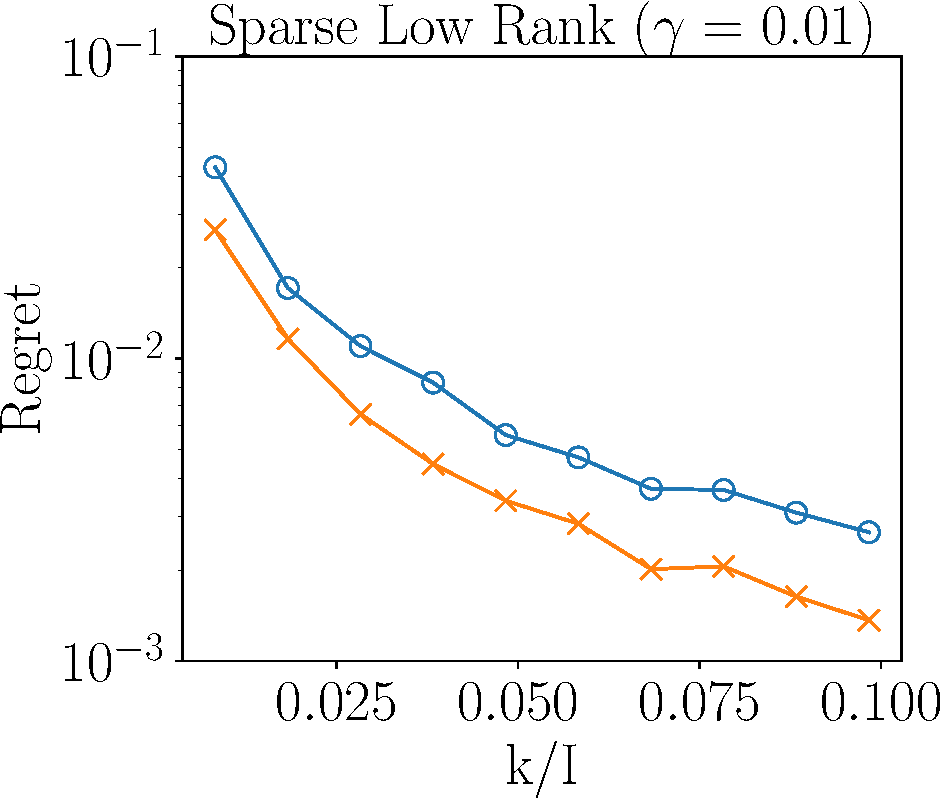
\includegraphics[scale = 0.24]{figure/fig3_slk_lnoise_600.pdf}
	\end{subfigure}
	\begin{subfigure}{0.3\textwidth}
		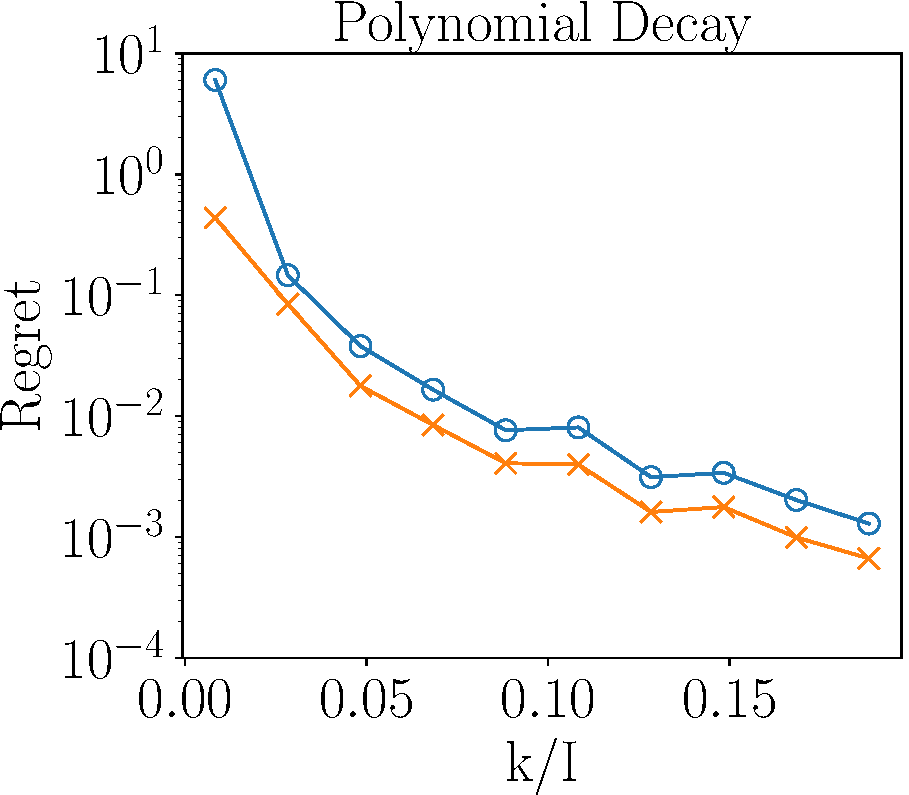
\includegraphics[scale = 0.24]{figure/fig3_spd_600.pdf}
	\end{subfigure}\\
	\begin{subfigure}{0.3\textwidth}
		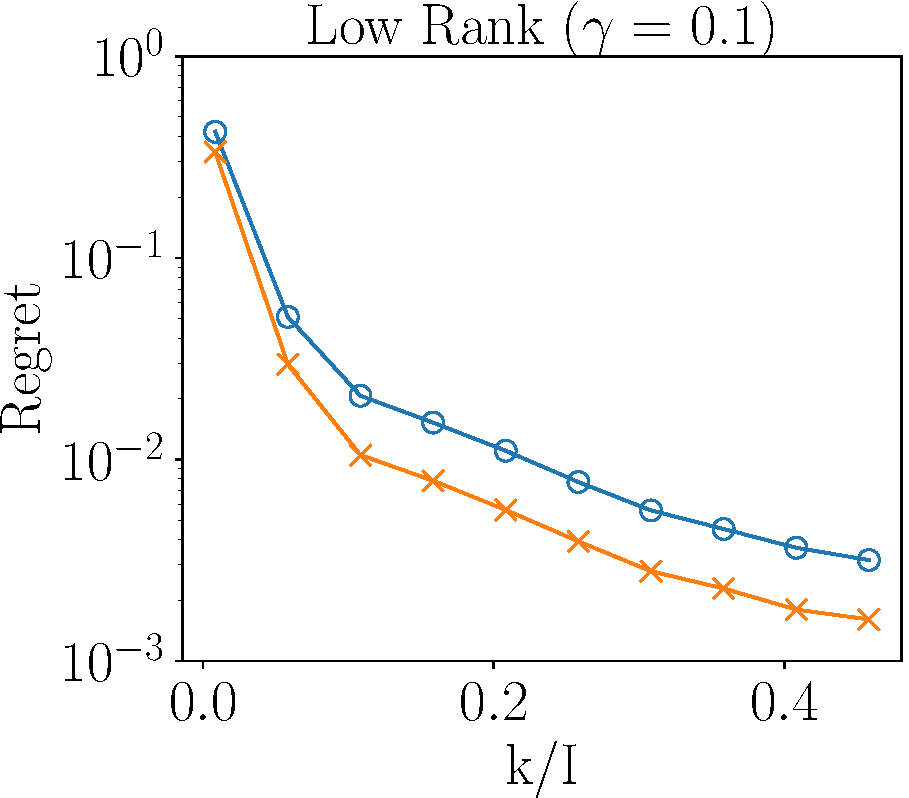
\includegraphics[scale = 0.24]{figure/fig3_lk_mnoise_600.pdf}
	\end{subfigure}
	\begin{subfigure}{0.55\textwidth}
		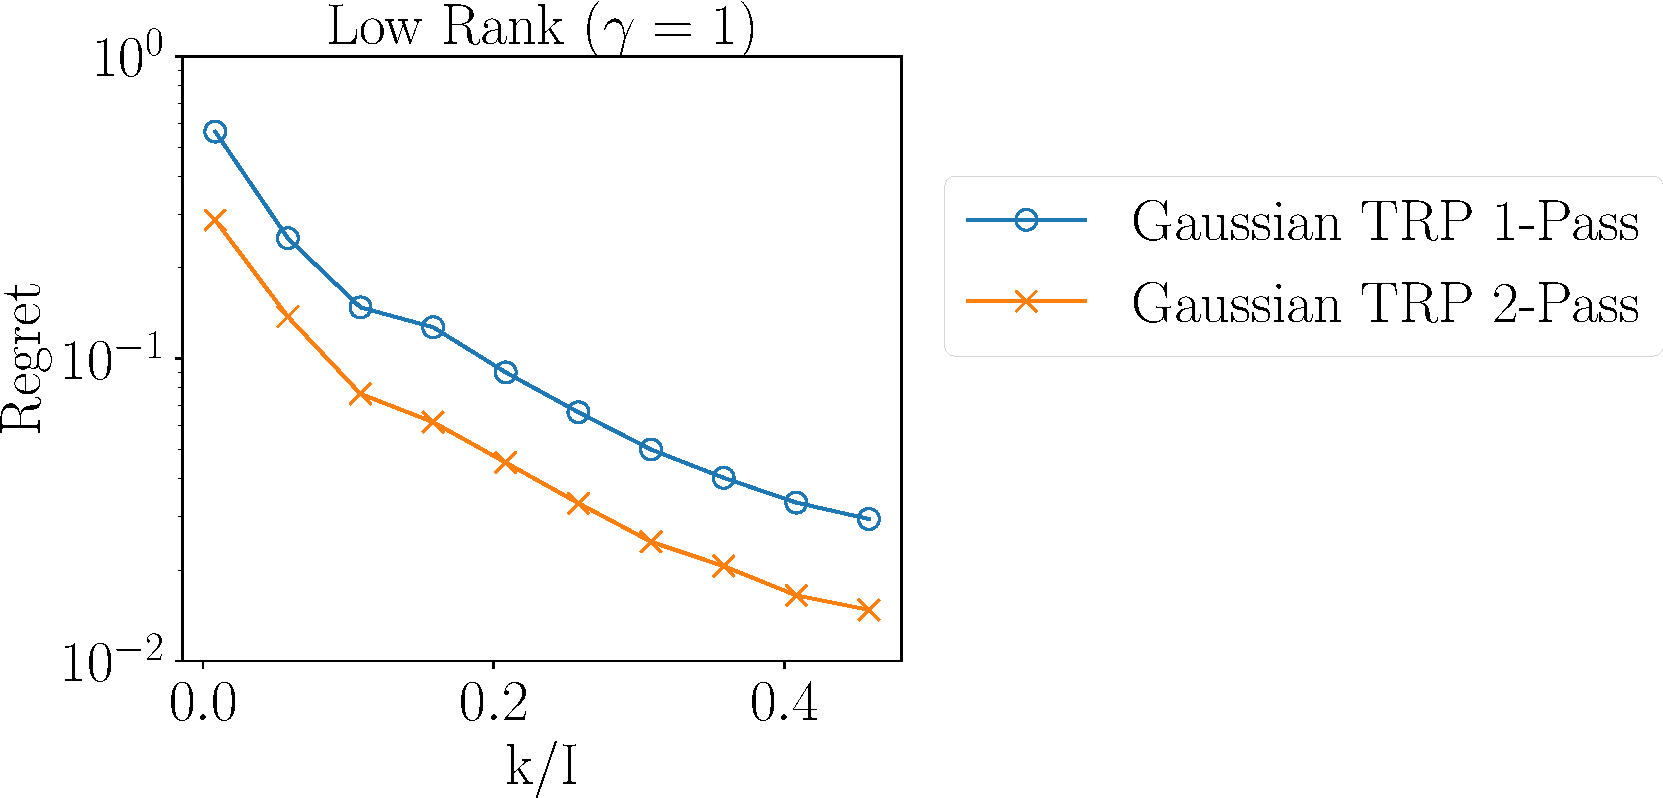
\includegraphics[scale = 0.24]{figure/fig3_lk_hnoise_600.pdf}
	\end{subfigure}
	\\
	\caption{\textit{Two-pass improves on one-pass.}
	We approximate 3D synthetic tensors (see \ref{s-synthetic-data}) with $I = 600$,
	using our one-pass and two-pass algorithms with $r = 5$ and varying $k$ ($s = 2k+1$),
	using the Gaussian TRP in the Tucker sketch.
	\label{fig:vary-k-600-compare}
  }
\end{figure}
In this section, we study the performance of our method.
We compare the performance of the method using various different
DRMs, including TRP.
We also compare our method with the algorithm proposed by \cite{malik2018low}
to show that for the same storage budget, our method produces better approximations.
Our two-pass algorithm outperforms the one-pass version, as expected.
(Contrast this to \cite{malik2018low}, where the multi-pass method
performs less well than the one-pass version.)
% Experiments on real data show effective compression
% can be achieved in a single pass.

\begin{figure}
	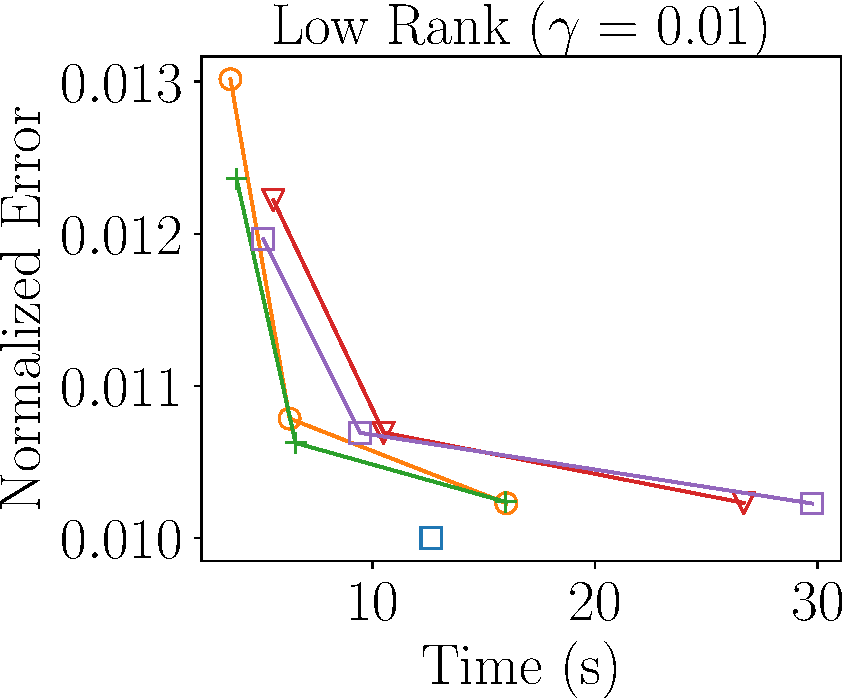
\includegraphics[height=2.5cm]{figure/lk_1pass_time.pdf}
	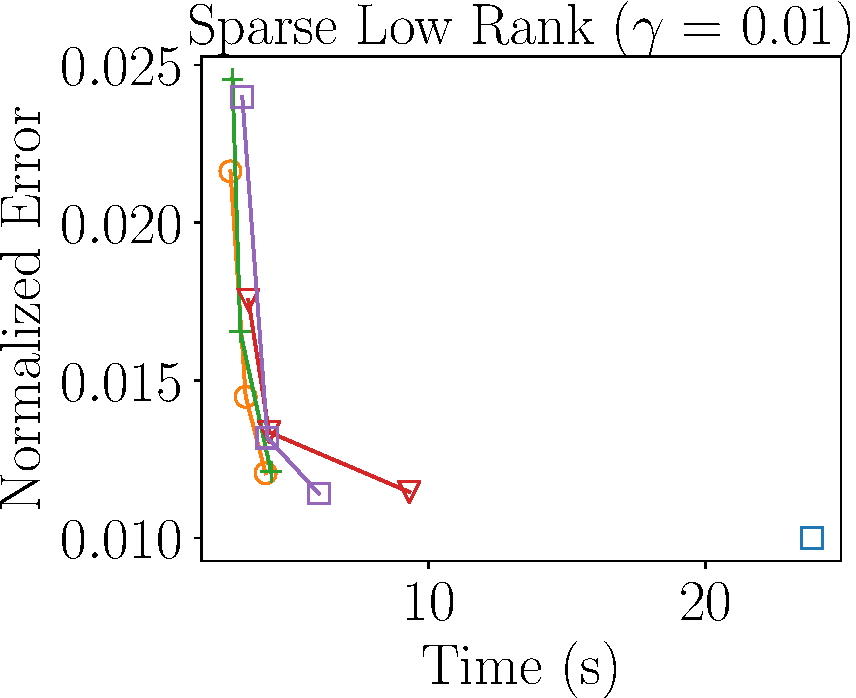
\includegraphics[height=2.5cm]{figure/slk_1pass_time.pdf}
	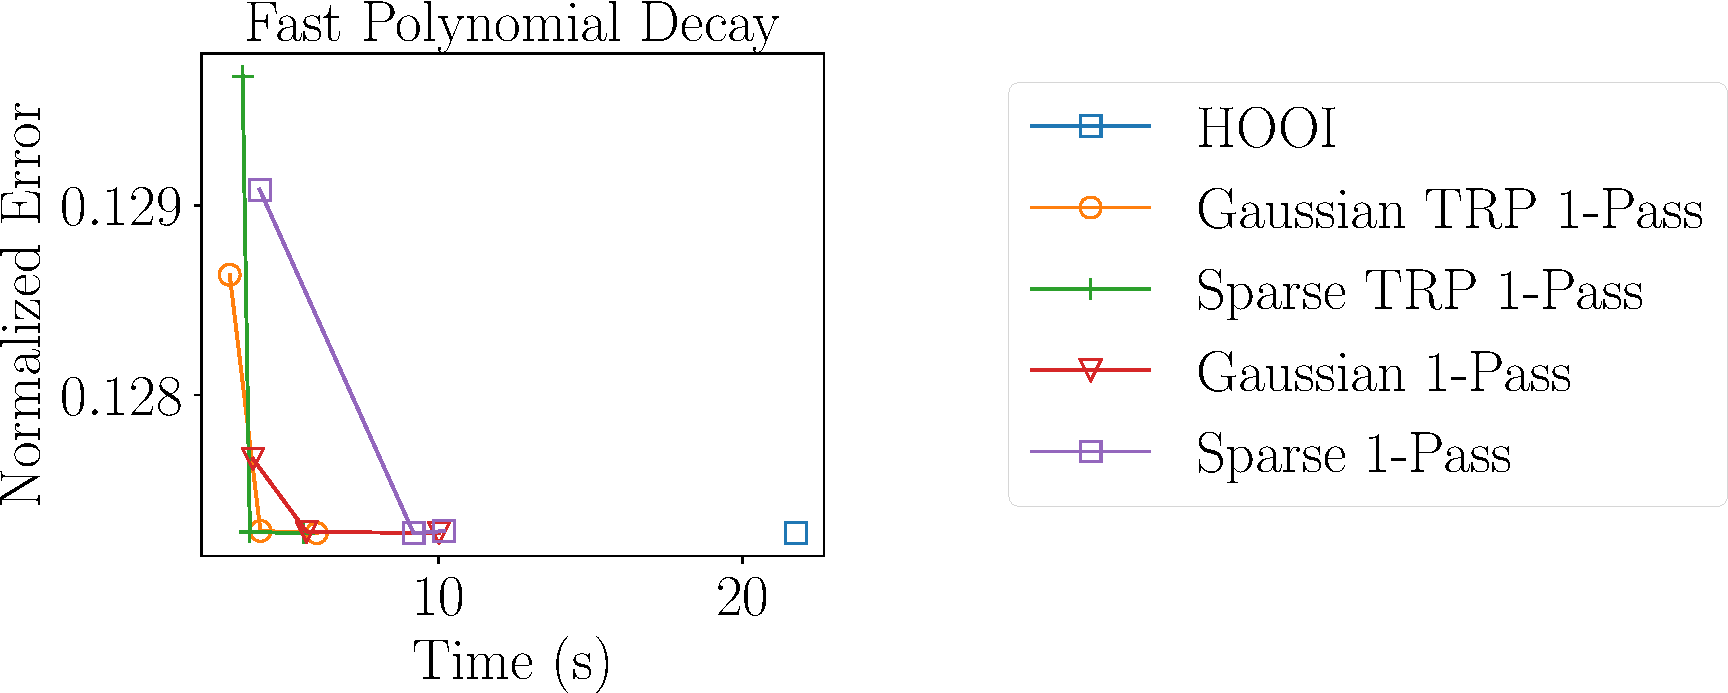
\includegraphics[height=2.5cm]{figure/fpd_1pass_time.pdf}\\
	\centering
	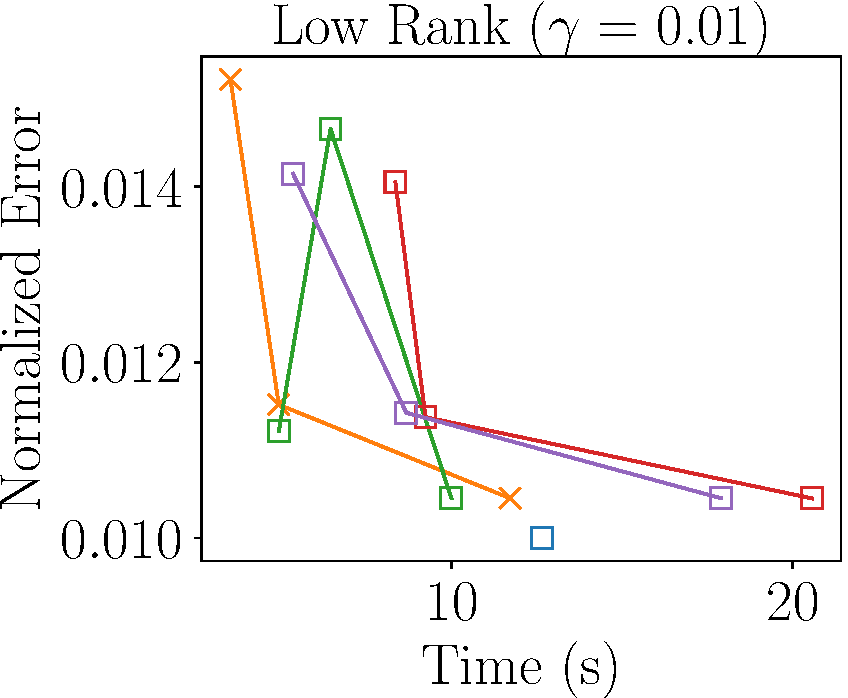
\includegraphics[height=2.5cm]{figure/lk_2pass_time.pdf}
	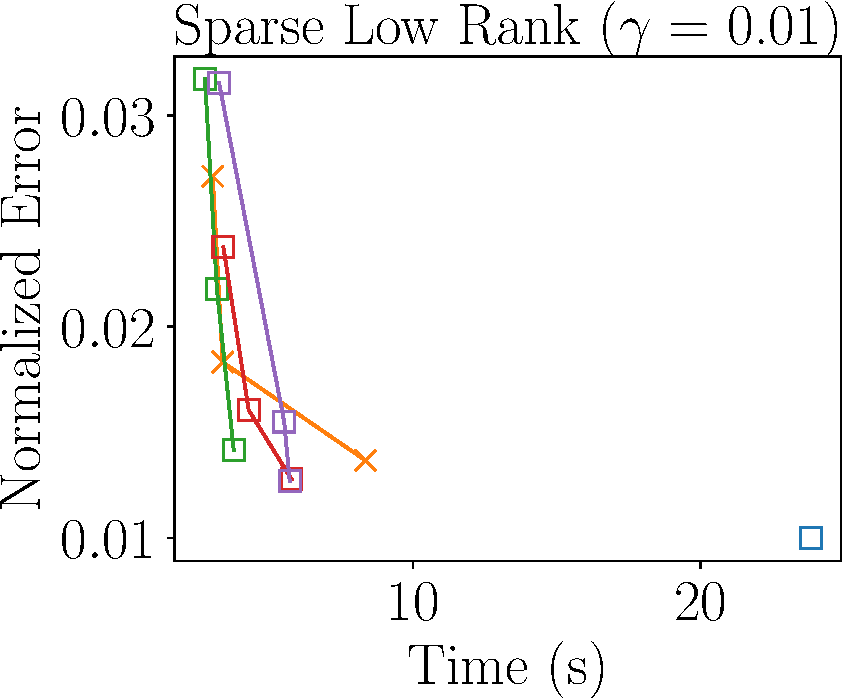
\includegraphics[height=2.5cm]{figure/slk_2pass_time.pdf}
	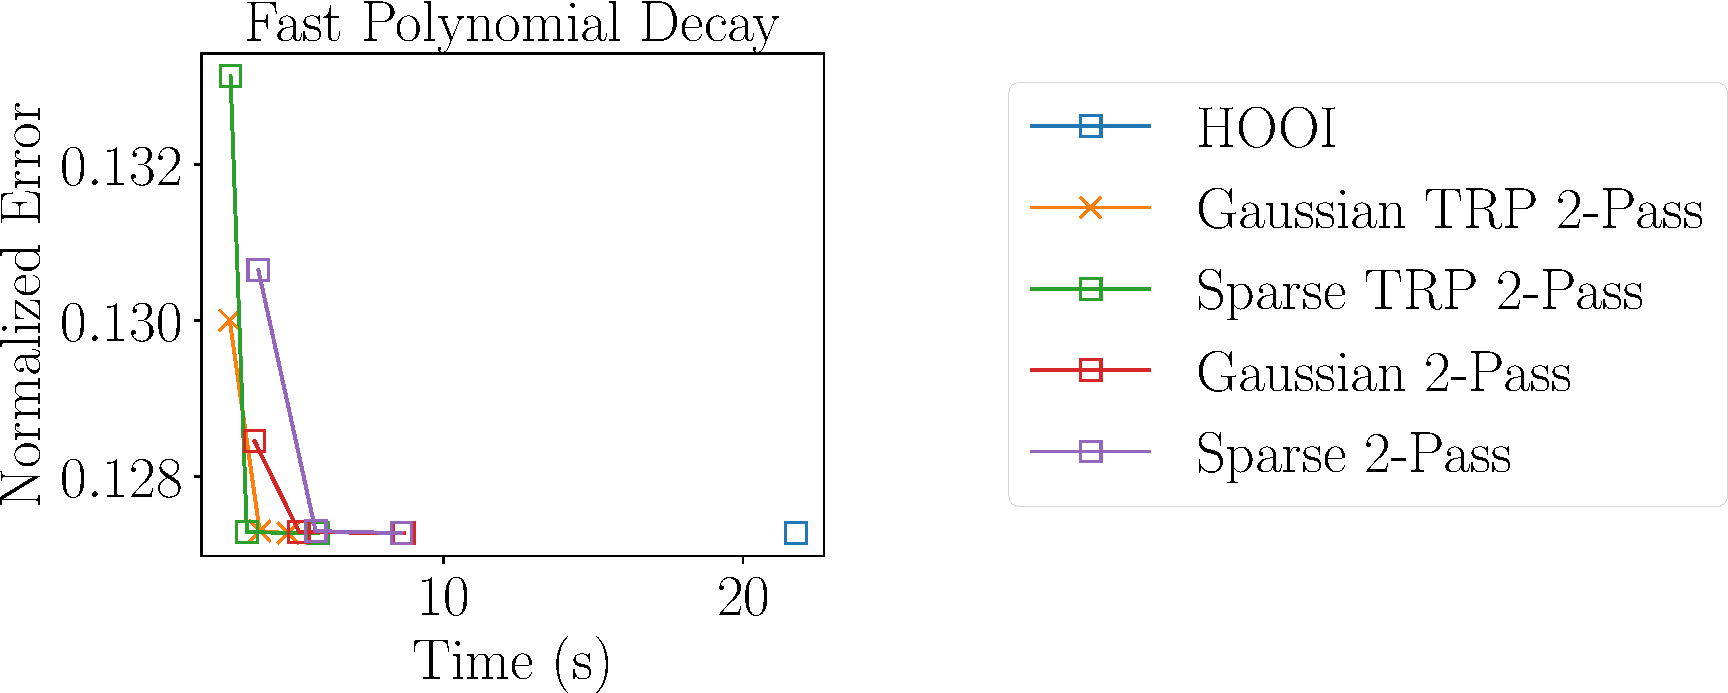
\includegraphics[height=2.5cm]{figure/fpd_2pass_time.pdf}\\
	\centering
	\caption{
	\textit{Faster approximations.}
	We approximate 3D synthetic tensors with $I = 600$ generated
	as described in \ref{s-synthetic-data},
	using HOOI and our one-pass and two-pass algorithms with $r = 5$
	for a few different $k$ ($s = 2k+1$).
	% We try several DRMs in the Tucker sketch:
	% Gaussian, Sparse, Gaussian TRP, and Sparse TRP.
	% Tradeoff between Time and Relative Error: We compare HOOI and our two algorithms across different random maps with $I=600, \mathbf{r}=(5,5,5)$, $\gamma = 0.01$.
}\label{fig:run_time}
\end{figure}

We evaluate the experimental results using two metrics:
\[
% \begin{array}{lc}
% \mbox{normalized error:} & \frac{\|\T{X} - \hat{\T{X}}\|_F}{\|\T{X}\|_F} \\
% \mbox{relative error:} & \frac{\|\T{X} - \hat{\T{X}}\|}{\|\T{X} - \T{X}_\text{HOOI}\|} - 1 \\
% \mbox{regret:} & \frac{\|\T{X} - \hat{\T{X}}\|_F}{\|\T{X}\|_F} -
%                    \frac{\|\T{X} - \T{X}_\text{HOOI}\|_F}{\|\T{X}\|_F}.
% \end{array}
\begin{array}{lc}
\mbox{normalized error:} & \|\T{X} - \hat{\T{X}}\|_F / \|\T{X}\|_F \\
% \mbox{relative error:} & \nicefrac{\|\T{X} - \hat{\T{X}}\|}{\|\T{X} - \T{X}_\text{HOOI}\|} - 1 \\
\mbox{regret:} & \left(\|\T{X} - \hat{\T{X}}\|_F - \|\T{X} - \T{X}_\text{HOOI}\|_F \right) / \|\T{X}\|_F.
\end{array}
\]
The normalized error measures the fraction of the energy in $\T{X}$
captured by the approximation.
The regret measures the increase in normalized error due to
using the approximation $\hat{\T{X}}$ rather than using $\T{X}_\text{HOOI}$.
The relative error measures the decrease in performance relative to HOOI.
%\mnote{Joel says: I prefer to call this the "normalized" error, rather than the "relative" error. The former scales the error so it should usually be less than one. The second compares the error with the "optimum" error: ||X - hat{X}|| / ||X - HOOI(X)|| - 1.You might consider whether you actually want the latter.}
The normalized error of a rank $\V{r}$ Tucker approximation $\hat{X}$
is always positive when $\T{X}$ has a larger rank.
In general, we find our proposed methods approaches the performance of HOOI
for large enough storage budgets.

We ran all experiments on a server with 128 Intel\textsuperscript{\textregistered} Xeon\textsuperscript{\textregistered} E7-4850 v4 2.10GHz CPU cores and 1056GB memory.
The code for our method is available at an anonymous Github repository \url{https://github.com/tensorsketch/tensorsketch}.

\subsection{Synthetic experiments}\label{s-synthetic-data}
All synthetic experiments use an input tensor with equal side lengths $I$.
We consider three different data generation schemes:
\begin{itemize}
\item \emph{Low rank + noise.} Generate a core tensor $\T{C} \in \mathbb{R}^{r^N}$ with entries drawn from $\mathrm{Unif}([0,1])$.
  Independently generate $N$ orthogonal factor matrices
  $\mathbf{A}_1, \dots, \mathbf{A}_N \in \mathbb{R}^{r \times I}$.
	Define $\T{X}^\natural = \T{C} \times_1 \mathbf{A}_1 \cdots \times_N \mathbf{A}_N$
	and the noise parameter $\gamma > 0$.
	Generate an input tensor as
	$\T{X} = \T{X}^\natural + (\gamma \|\T{X}^\natural\|_F / I^{N/2})\T{\epsilon}$
	where the noise $\T{\epsilon}$ has i.i.d. $\mathcal{N}(0,1)$ entries.
	% by orthogonalizing random matrices with each entry drawn from $\mathcal{N}(0,1)$.
%   The input tensor is
%  \[
% \T{X} = \T{C} \times_1 \mathbf{A}_1 \cdots \times_N \mathbf{A}_N + \sqrt{\frac{\gamma^2 \cdot \|\T{X}^\natural\|_F^2}{I^N}} \mathcal{N}(0,1),
% \]
% where $\T{X}^\natural = \T{C} \times_1 \mathbf{A}_1 \cdots \times_N \mathbf{A}_N$.
% Here $1/\gamma^2$ measures the signal-to-noise ratio.
% In the simulations, we use three different noise levels: $\gamma = 0.01, 0.1, 1$.
\item \emph{Sparse low rank + noise.} We construct the input tensor $\T{X}$ as above (Low Rank + Noise),
but with sparse factor matrices $\mathbf{A}_n$:
If $\delta_n$ is the sparsity (proportion of non-zero elements) of $\mathbf{A}_n$,
then the sparsity of the true signal $\T{X}^\natural$ is $\prod_{n=1}^N \delta_n$.
%We set the noise $\gamma = 0.01$ (Results for $\gamma = 0.1,0.1$ are empirically analogous to the previous setting).
We use $\delta_n = 0.2$ unless otherwise specified.
\item \emph{Polynomial decay.} We construct the input tensor $\T{X}$ as
  \begin{equation*}
      \T{X} = \mathop{\textbf{superdiag}}(1,\dots,1, 2^{-t},3^{-t},\dots, (I-r)^{-t}).
  \end{equation*}
  The first $r$ entries are 1.
	Recall $\mathop{\textbf{superdiag}}$ converts a vector to $N$ dimensional superdiagonal tensor.
  Our experiments use $t = 1$ (geometric decay).
\end{itemize}

\subsubsection{Different dimension reduction maps perform similarly}
Our first experiment investigates the performance of our one-pass fixed-rank algorithm
as the sketch size (and hence, required storage) varies,
for several types of dimension reductions maps, including Gaussian, SSRFT, Gaussian TRP, and Sparse TRP.
We generate synthetic data as described above with $\mathbf{r} = (5,5,5), I = 600$.
\ref{fig:vary-k-600} shows the rank-$\mathbf{r}$ approximation error
as a function of the compression factor $k/I$.
\ifdefined \issupplement
(Results for other input tensors appear in the supplement.)
\else
(Results for other input tensors are presented as
\ref{fig:vary-k-400-app} and \ref{fig:vary-k-200-app} in \ref{appendix:more_result}.)
\fi
We see that the log relative error for our one-pass algorithm
converges to that of HOOI as $k$ increases for all input tensors.
In the low rank case, the convergence rate is lower for higher noise levels.
In general, the performance for different maps are approximately the same,
although our theory only pertains to the Gaussian map.
% In the low-rank sparse case and low-rank high noise case,
% the Gaussian TRP outperforms the Gaussian, possibly due to the implicit bias from the Khatri-Rao structure.

We evaluate the run time for HOOI and our two algorithms with several different DRMs in \ref{fig:run_time}. We can see that the one-pass algorithm is always slightly faster than the two-pass algorithm. The TRP generally provides a modest speedup in addition to the memory advantage.
Both our one-pass and two-pass algorithms achieve nearly the accuracy of HOOI,
and are usually much faster. % for tensors that are not exactly low rank.

\begin{figure}
	\centering
	\begin{subfigure}{0.3\textwidth}
		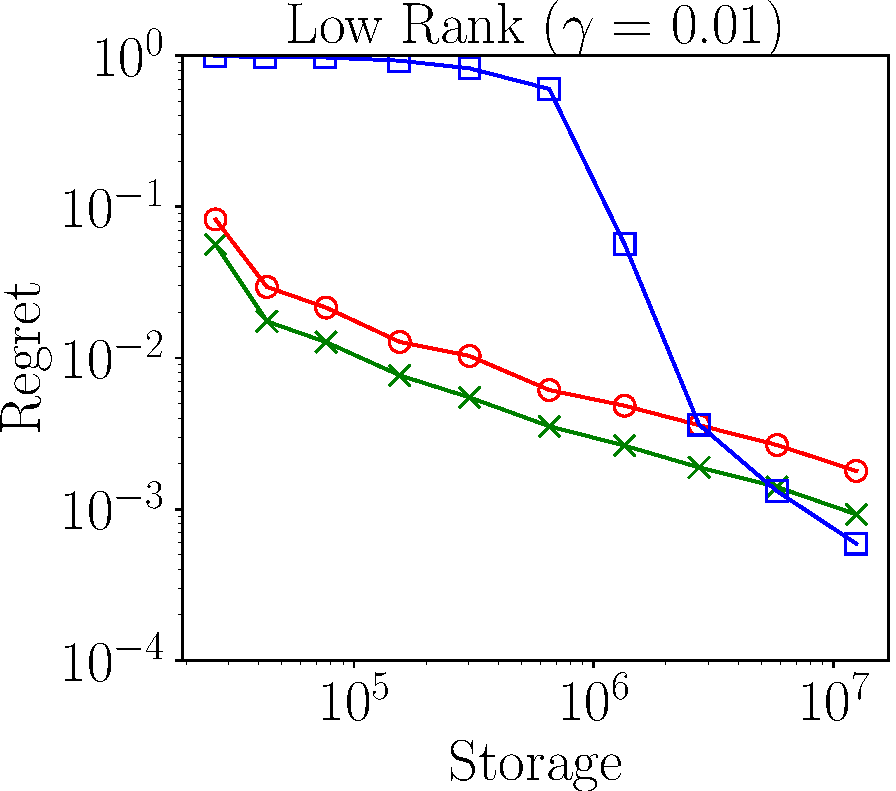
\includegraphics[scale = 0.24]{figure/fig1_lk_lnoise.pdf}
	\end{subfigure}
	\begin{subfigure}{0.3\textwidth}
		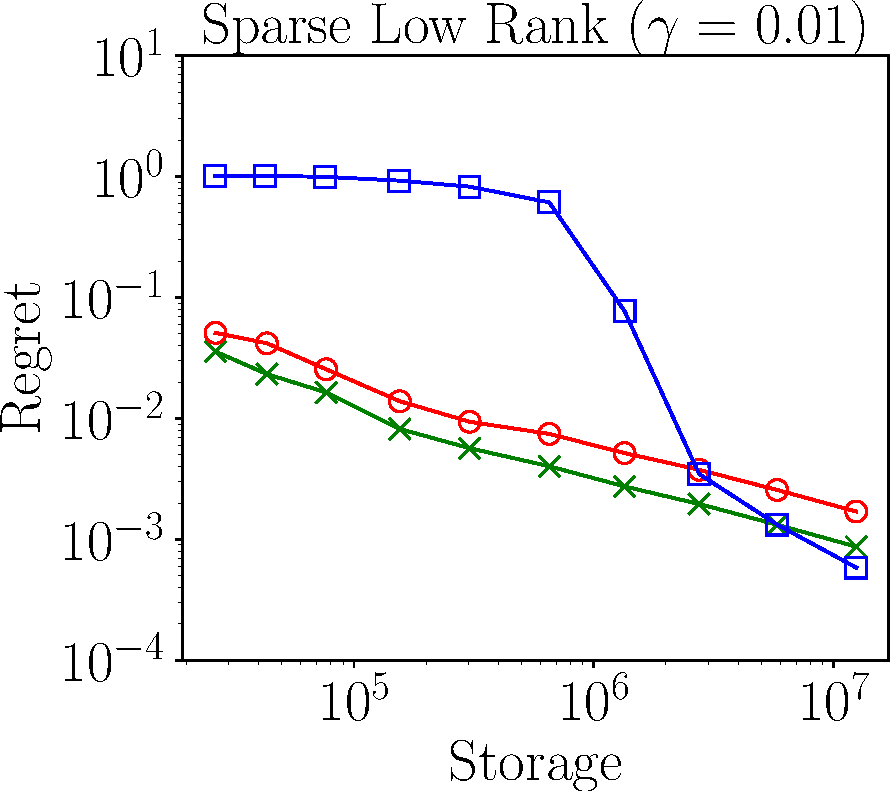
\includegraphics[scale = 0.24]{figure/fig1_slk_lnoise.pdf}
	\end{subfigure}
	\begin{subfigure}{0.3\textwidth}
		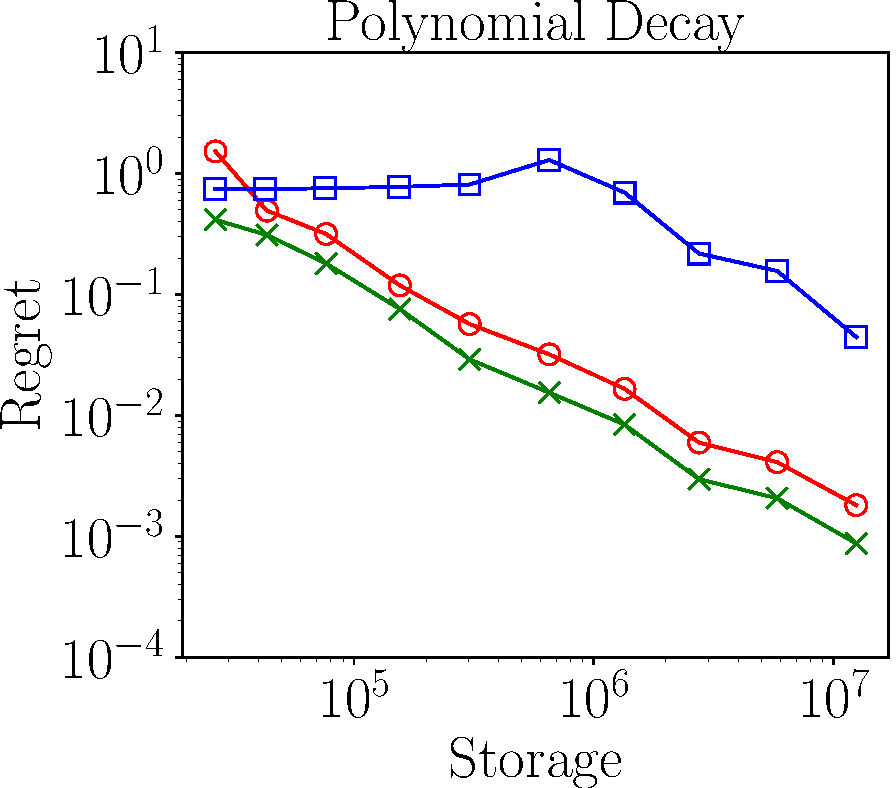
\includegraphics[scale = 0.24]{figure/fig1_spd.pdf}
	\end{subfigure}\\
	\begin{subfigure}{0.3\textwidth}
		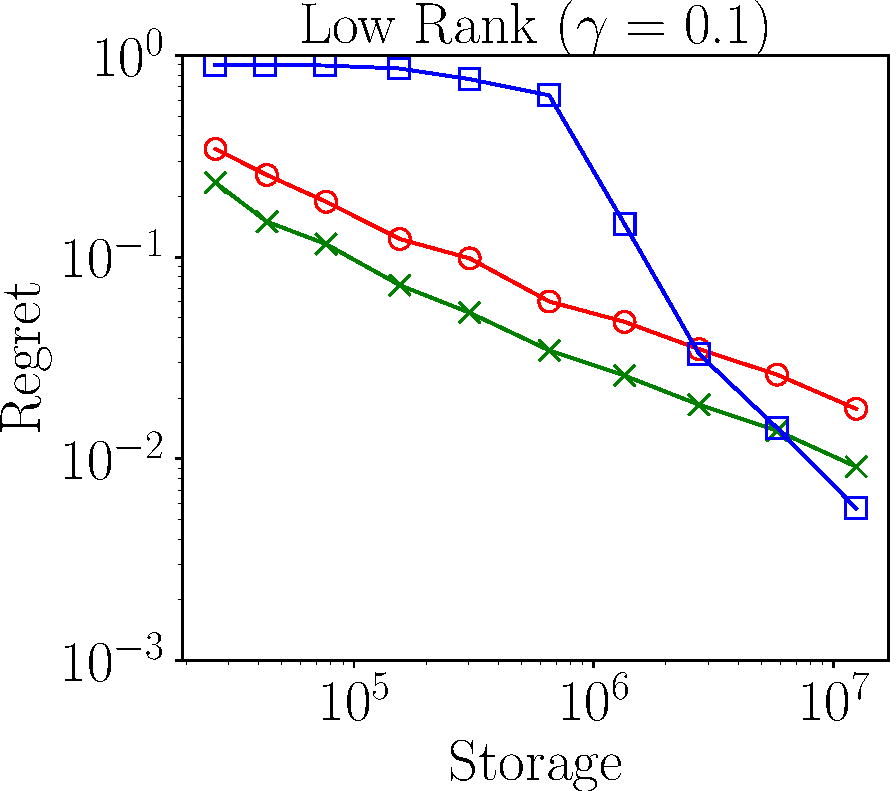
\includegraphics[scale = 0.24]{figure/fig1_lk_mnoise.pdf}
	\end{subfigure}
	\begin{subfigure}{0.43\textwidth}
		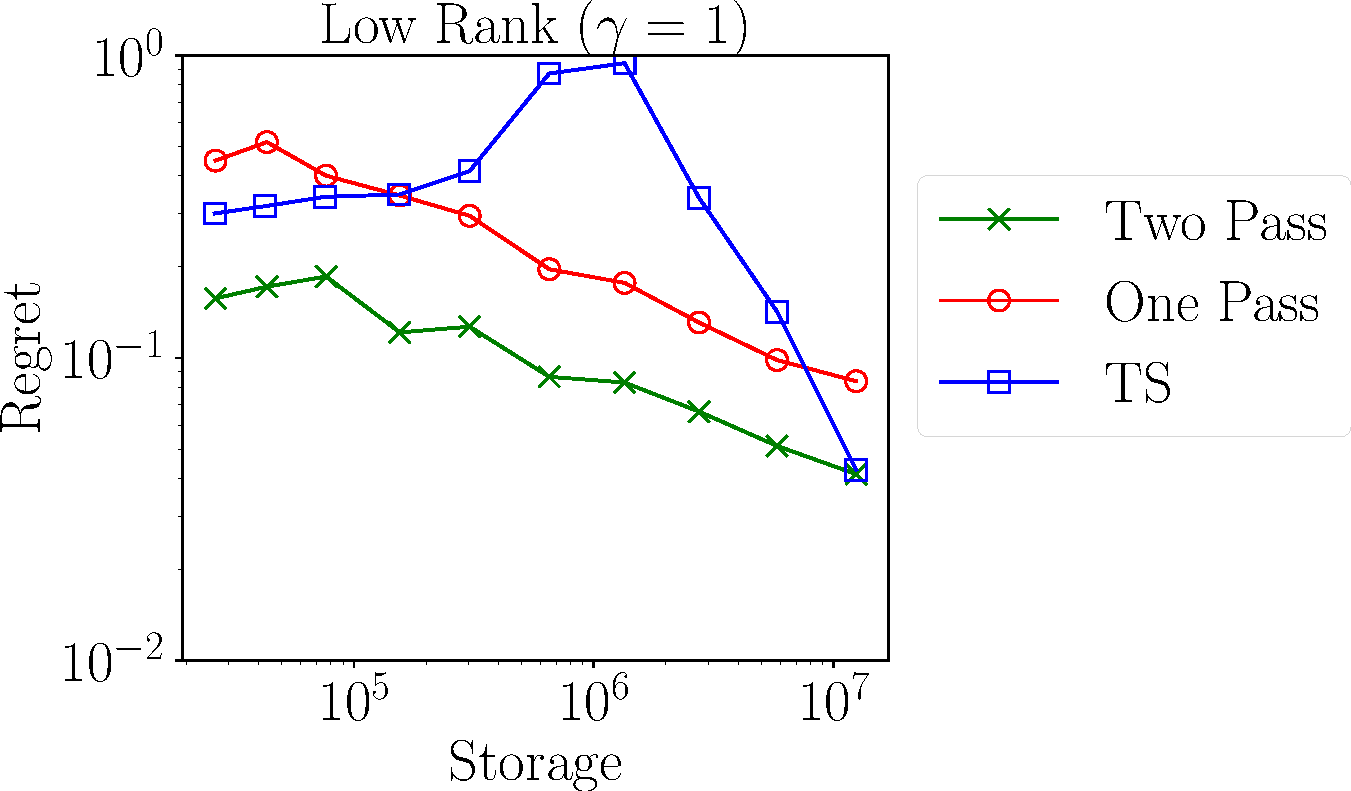
\includegraphics[scale = 0.24]{figure/fig1_lk_hnoise.pdf}
	\end{subfigure}\\
	\caption{\textit{Approximations improve with more memory: synthetic data.}
	We approximate 3D synthetic tensors (see \ref{s-synthetic-data}) with $I = 300$,
	using  T.-TS and our one-pass and two-pass algorithms
	with the Gaussian TRP to produce approximations with equal ranks $r=10$.
	Notice every marker on the plot corresponds to a 2700$\times$ compression!}\label{fig:vary-memory}
	% The total memory use is determined by the sketch size,
	% computed as $((2k+1)^N + kIN)$ for the one-pass method and $(Kr^{2N}+Kr^{2N-2})$ for T.-TS.
\end{figure}

\begin{figure}
	\centering
	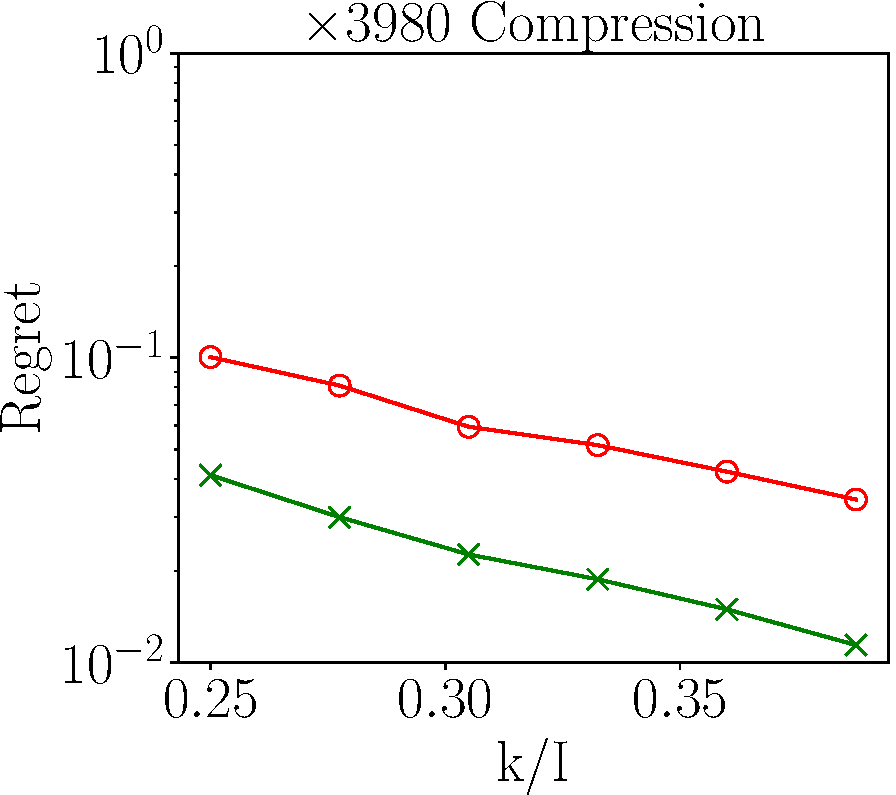
\includegraphics[height=2.9cm]{figure/multi_ABSORB_frk8.pdf}
	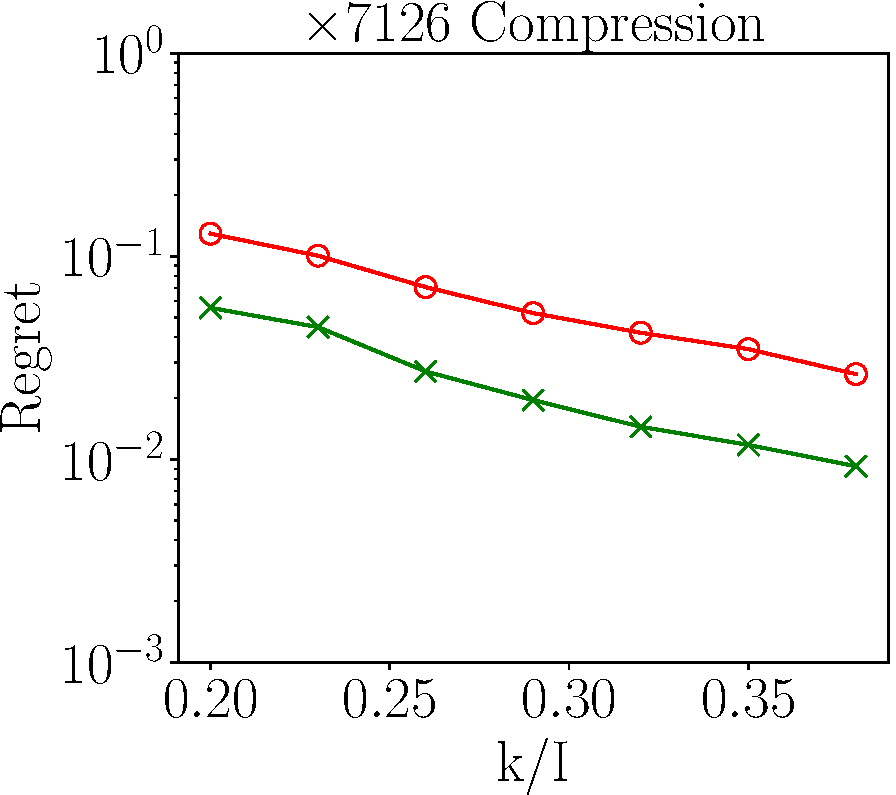
\includegraphics[height=2.9cm]{figure/multi_ABSORB_frk10.pdf}
	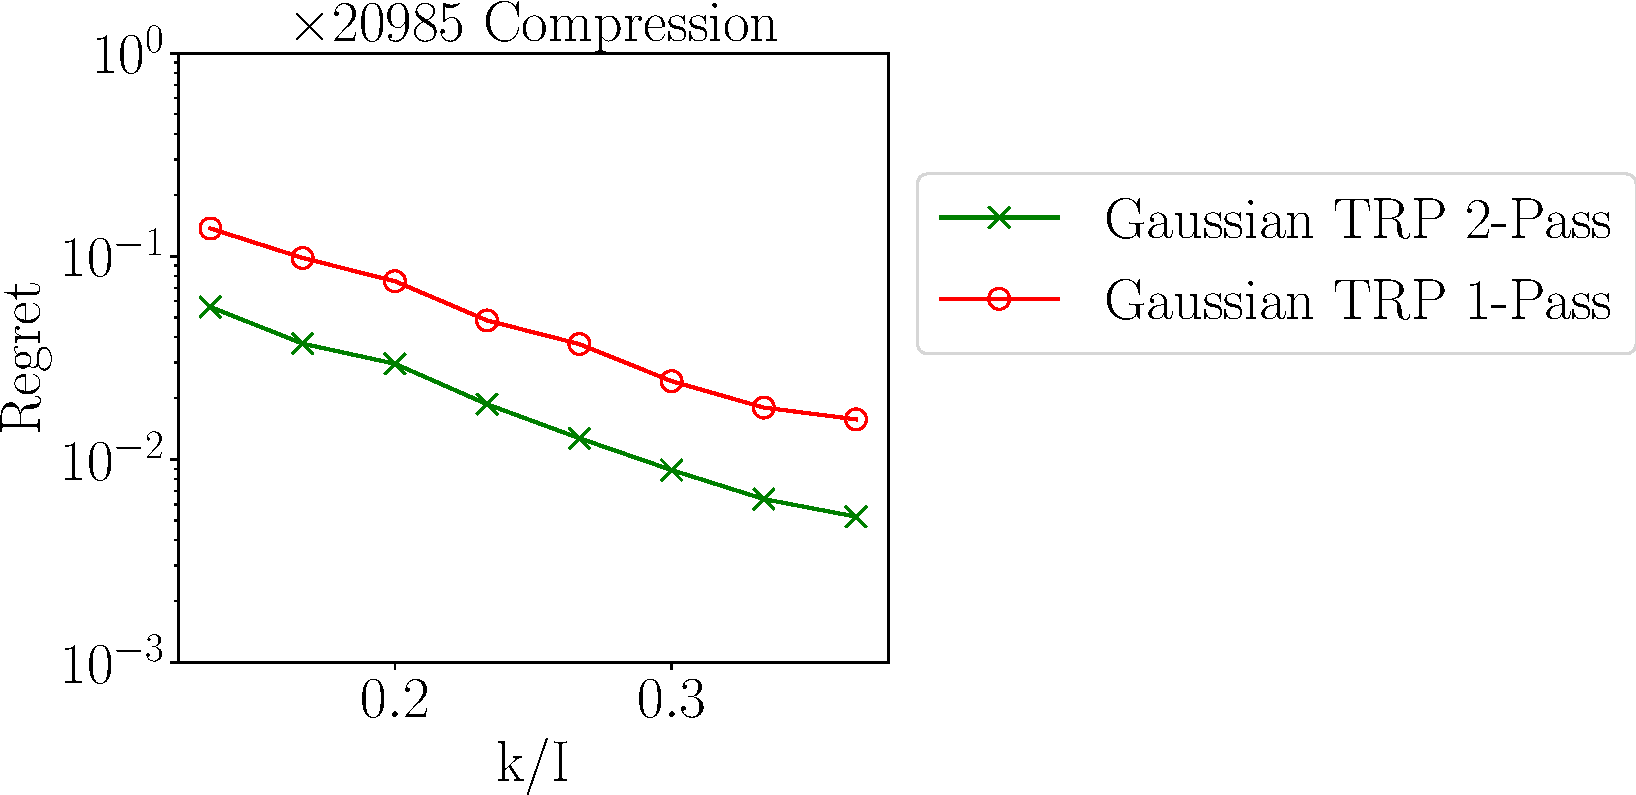
\includegraphics[height=2.9cm]{figure/multi_ABSORB_frk15.pdf}\\
	\textbf{Aerosol Absorption}\\~\\
	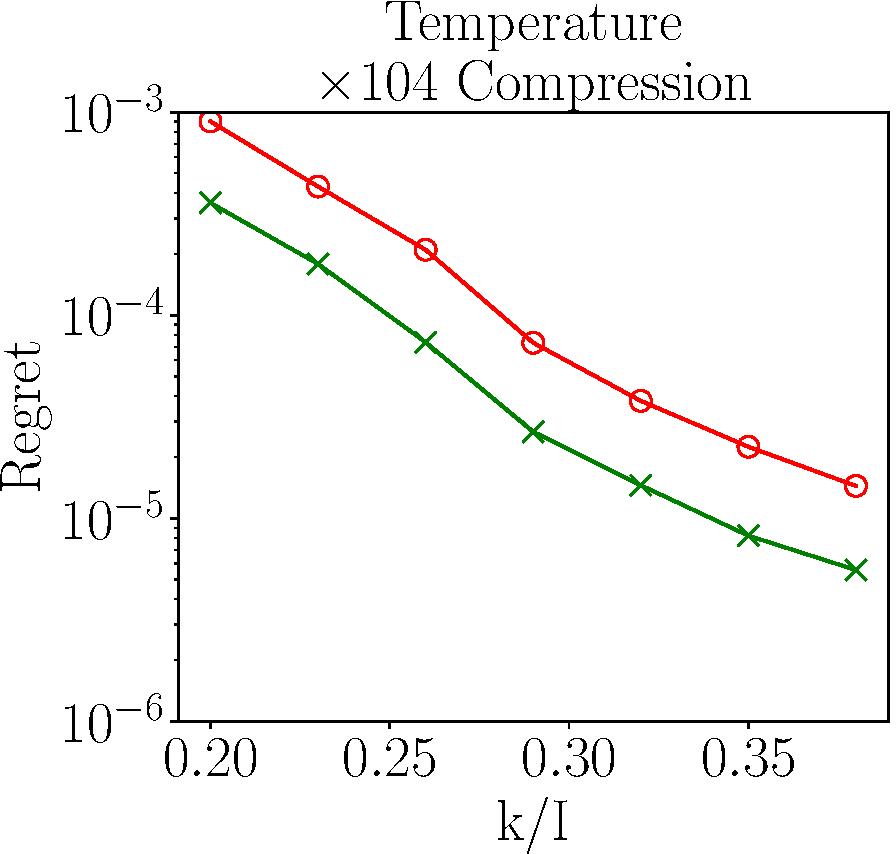
\includegraphics[height=2.9cm]{figure/multi_T_frk10.pdf}
	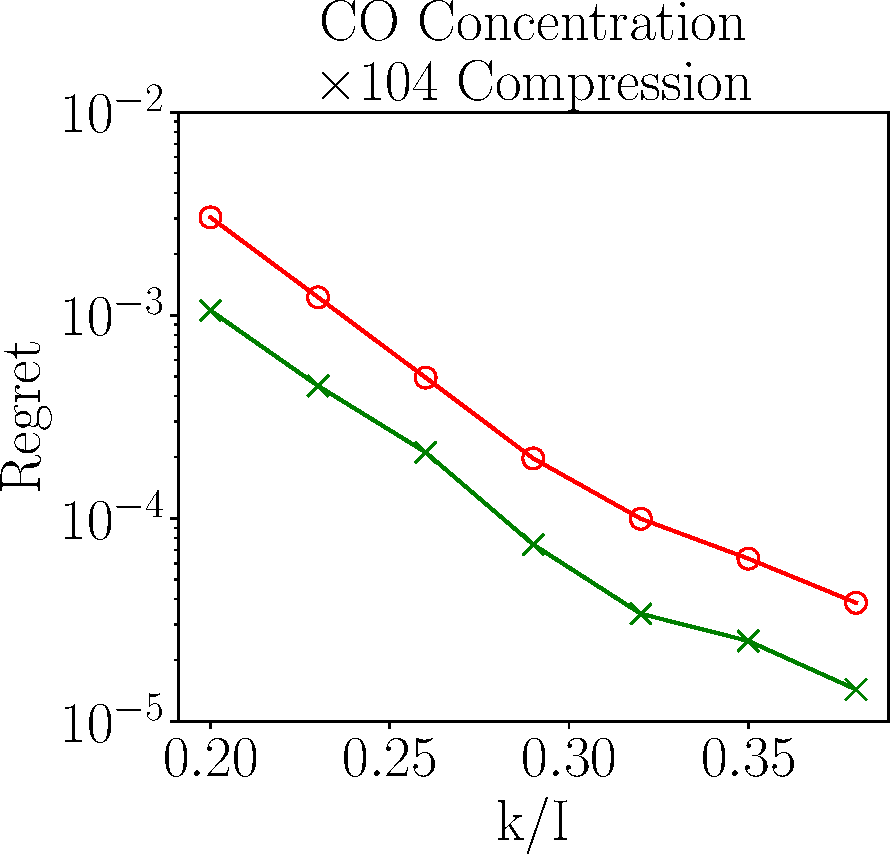
\includegraphics[height=2.9cm]{figure/multi_CO_frk10.pdf}
	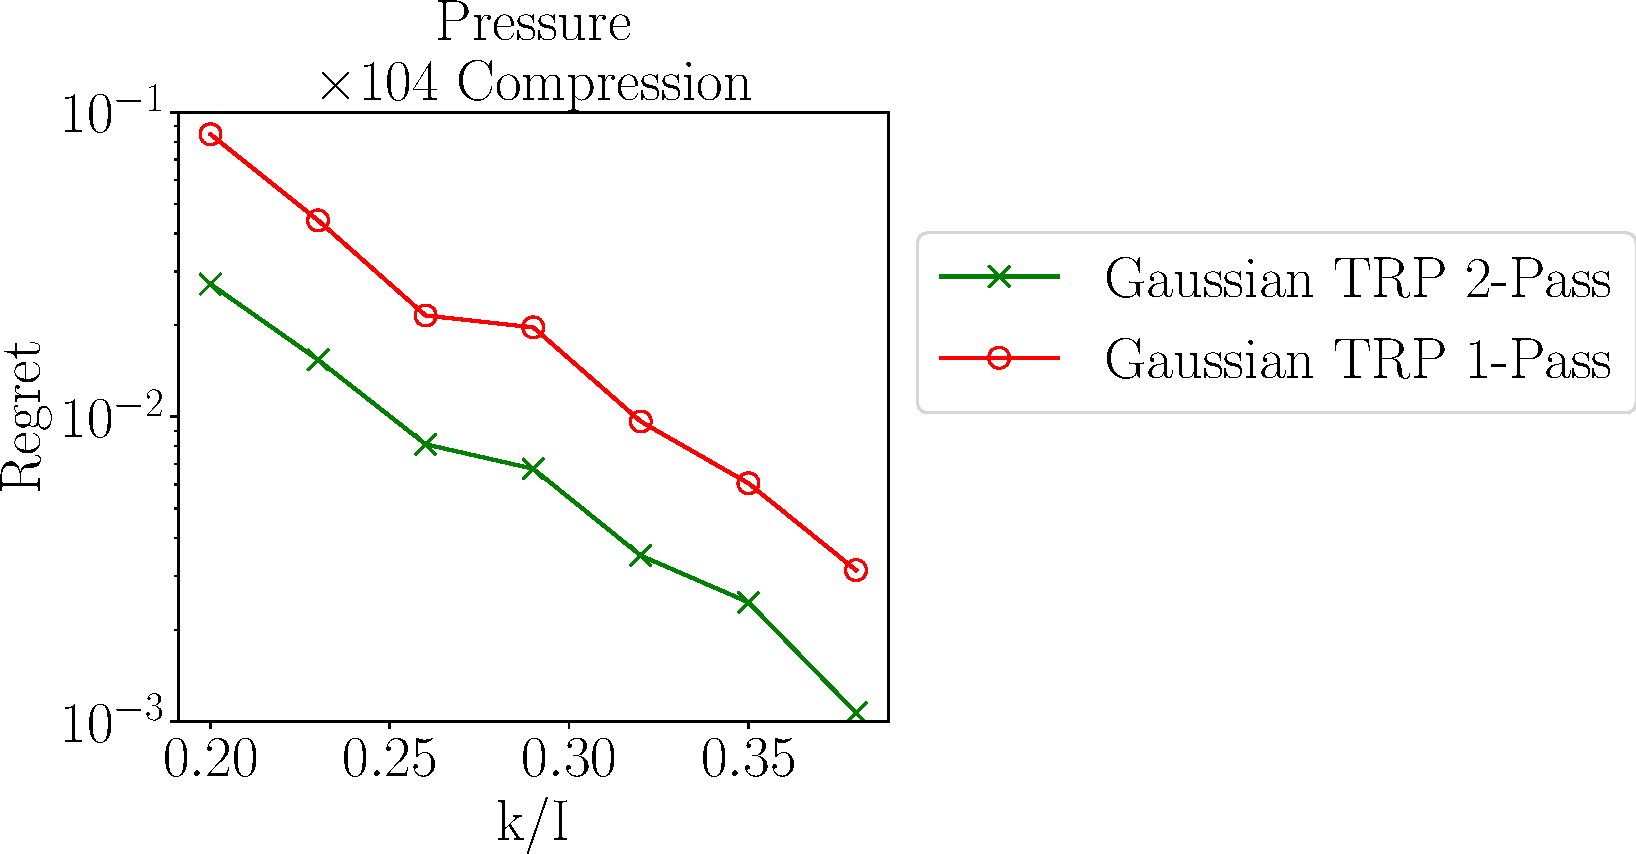
\includegraphics[height=2.9cm]{figure/multi_P_frk10.pdf}\\
	\textbf{Combustion Simulation}\\
	\caption{\textit{Approximations improves with more memory: real data.}
		% The aerosol absorption data	($240 \times 30 \times 192 \times 288$) is from CESM CAM 5.0.
		% The combustion data %for pressure, CO concentration, and temperature
		% (all of size $1408 \times 128 \times 128$)
		% is from \cite{lapointe2015differential}.
		We approximate aerosol absorption and combustion data
		using our one-pass and two-pass algorithms with the Gaussian TRP.
		We compare three target ranks ($r/I = 0.125,0.1,0.067$) for the former,
		and use the same target rank ($r/I = 0.1$) for each measured quantity in
		the combustion dataset.
		Notice $r/I = 0.1$ gives a hundred-fold compression!
	}\label{fig:climate}
\end{figure}

\begin{figure}[h!]
	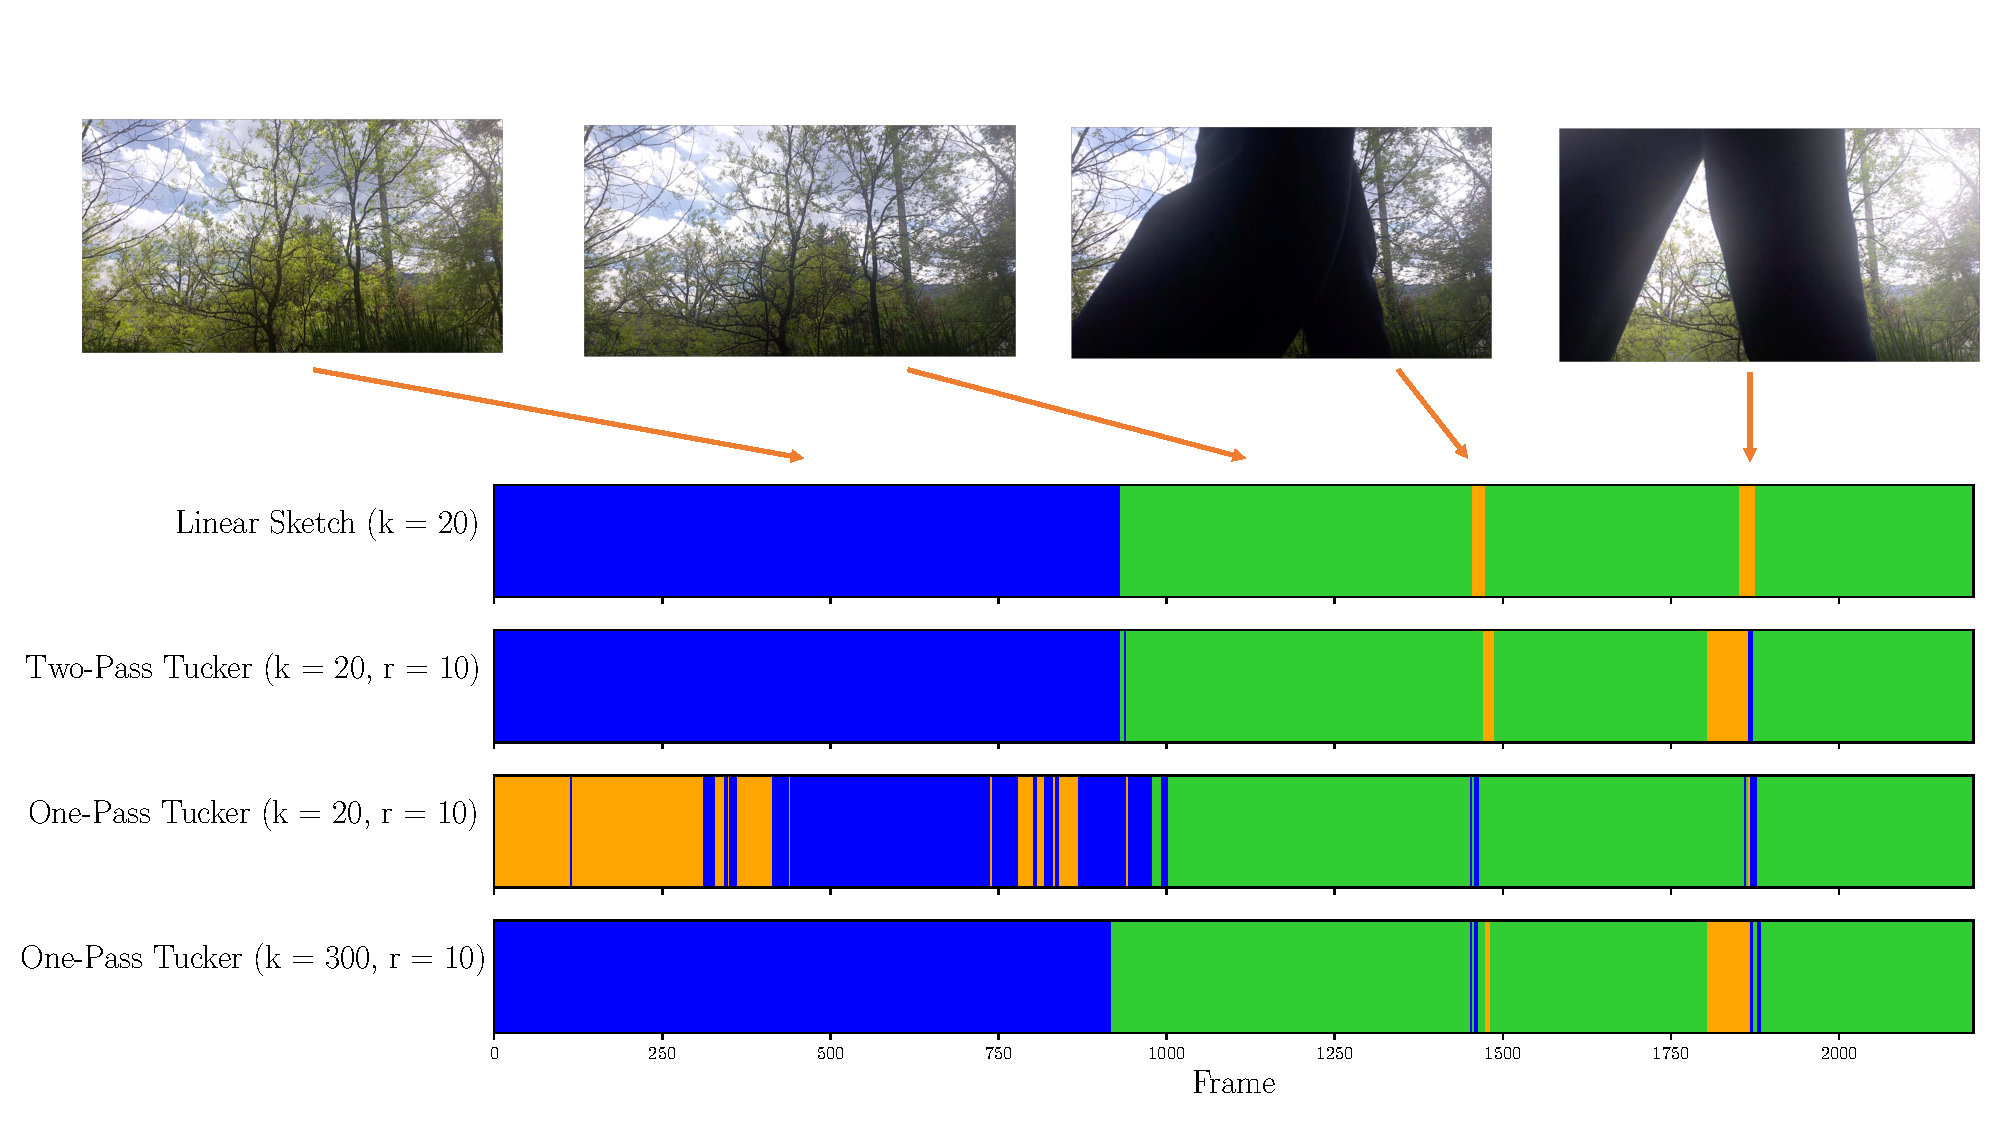
\includegraphics[height=7cm]{figure/video_classification_result.pdf} \\
	\centering
	\textbf{Video Scene Classification}
	\caption{\textit{Video Scene Classification}
		($2200 \times 1080 \times 1980$):
		We classify frames from the video data
		from \cite{malik2018low} (collected as a third order tensor with size $2200 \times 1080 \times 1980$) using $K$-means with $K$=3 on vectors computed using four different methods. $s = 2k+1$ throughout.
		1) The linear sketch along the time dimension (Row 1).
		2-3) the Tucker factor along the time dimension,
		computed via our two-pass (Row 2) and one-pass (Row 3) algorithms.
		%with parameters $r=10$, $k = 20$, and $s = 41$.
		4) The Tucker factor along the time dimension,
		computed via our one-pass (Row 4) algorithm
		%with parameters $r=10$, $k = 300$, and $s = 601$.
		}\label{fig:video}
\end{figure}

\begin{figure}[h!]
	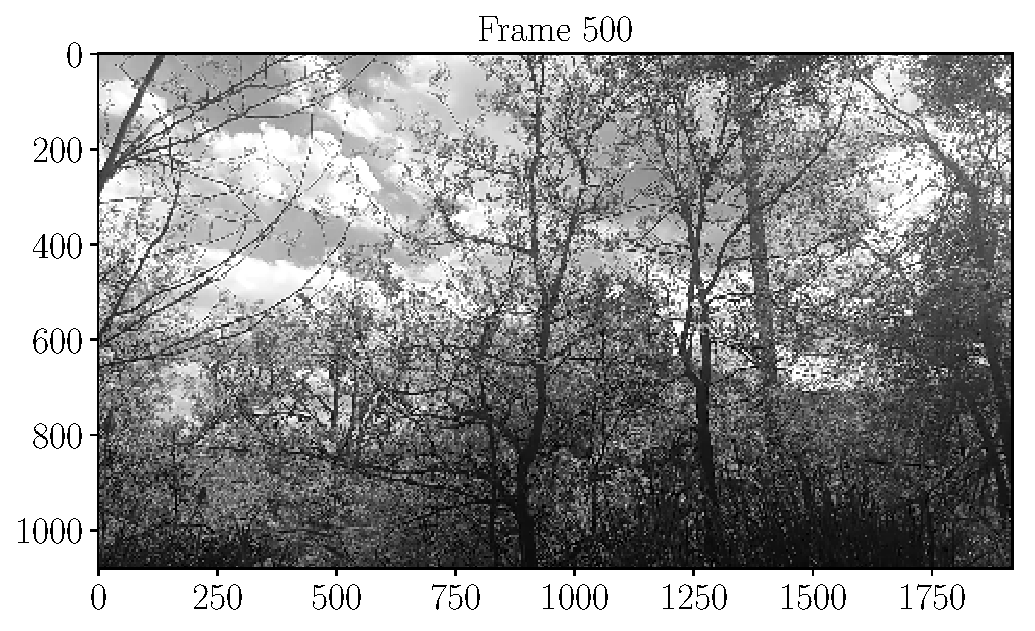
\includegraphics[height=2.4cm]{figure/frame500.pdf}
	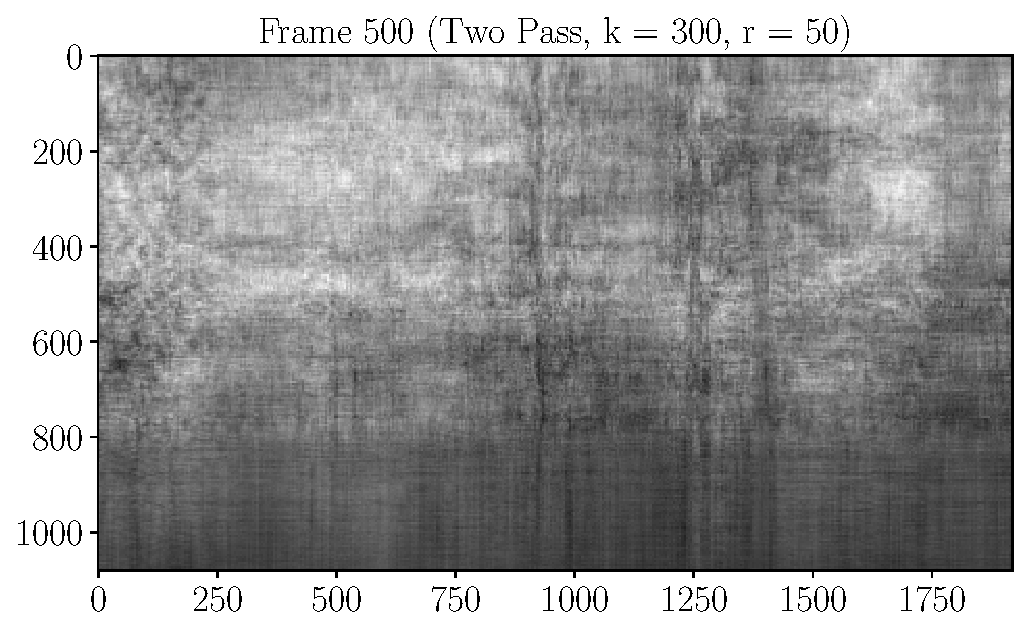
\includegraphics[height=2.4cm]{figure/2pass_k300_r50_frame500.pdf}
	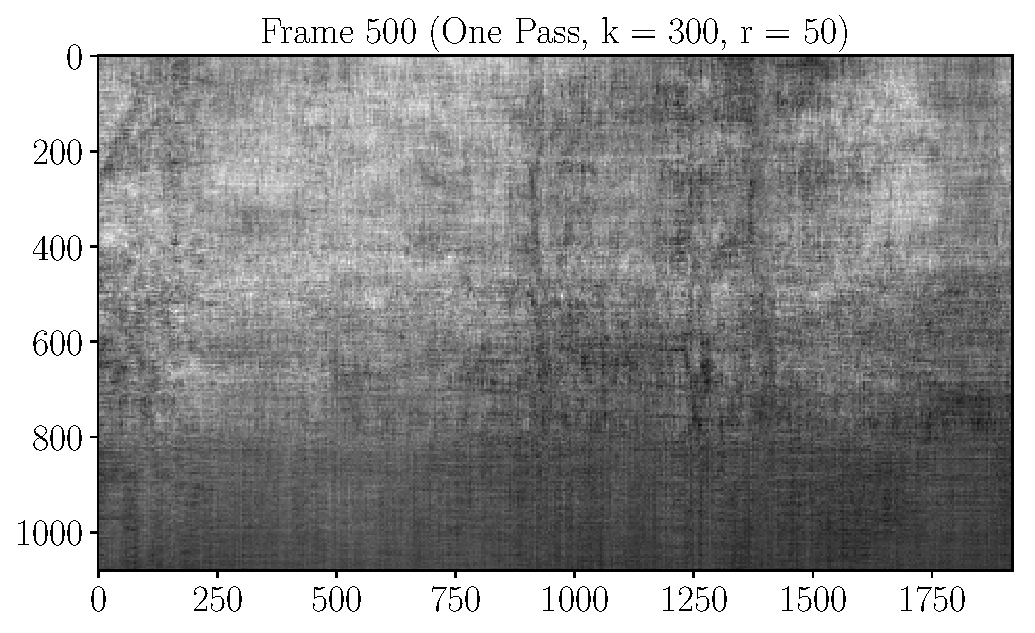
\includegraphics[height=2.4cm]{figure/1pass_k300_r50_frame500.pdf}
	\centering
	\caption{\textit{Visualizing Video Recovery:}
	Original frame (left);
	approximation by two-pass sketch (middle);
	approximation by one-pass sketch (right).
	% Frame 500
	}\label{fig:Frame500}
\end{figure}

\begin{figure}[h!]
	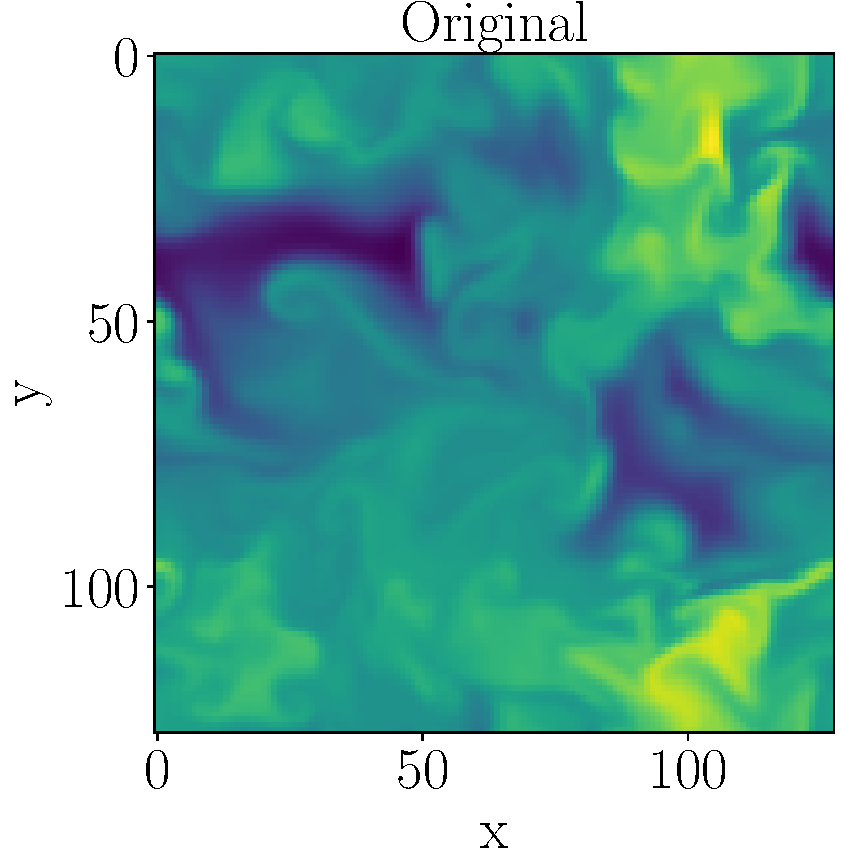
\includegraphics[height=3cm]{figure/T100_original.pdf}
	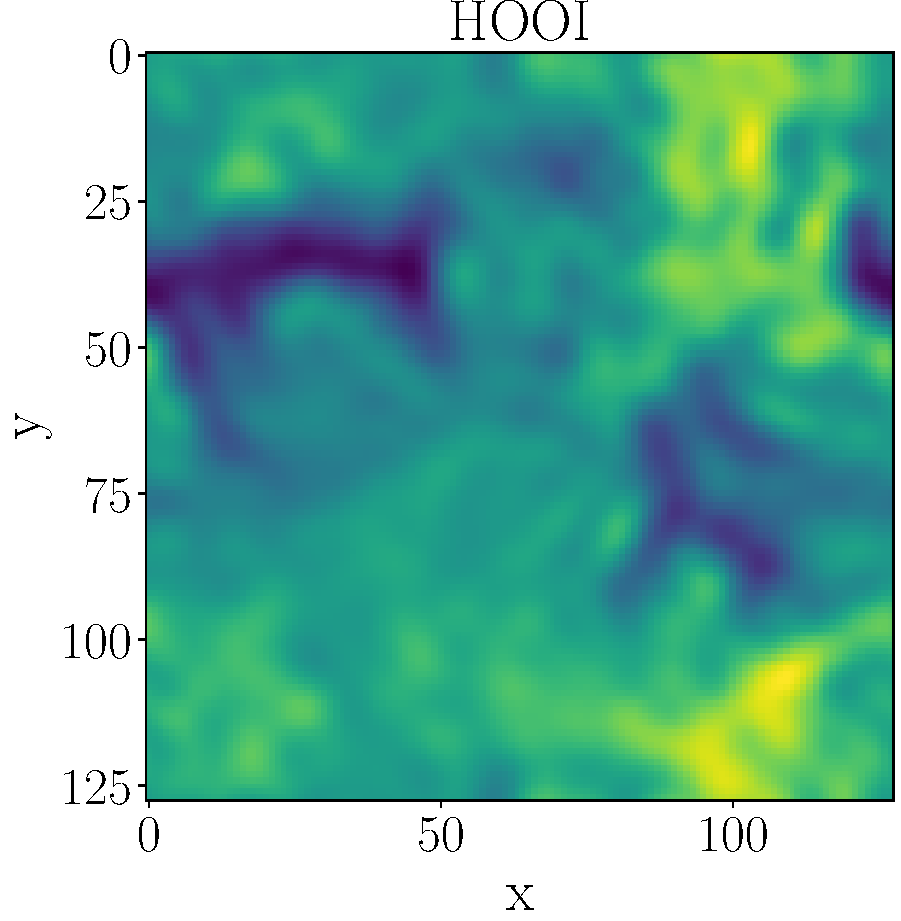
\includegraphics[height=3cm]{figure/T100_hooi.pdf}
	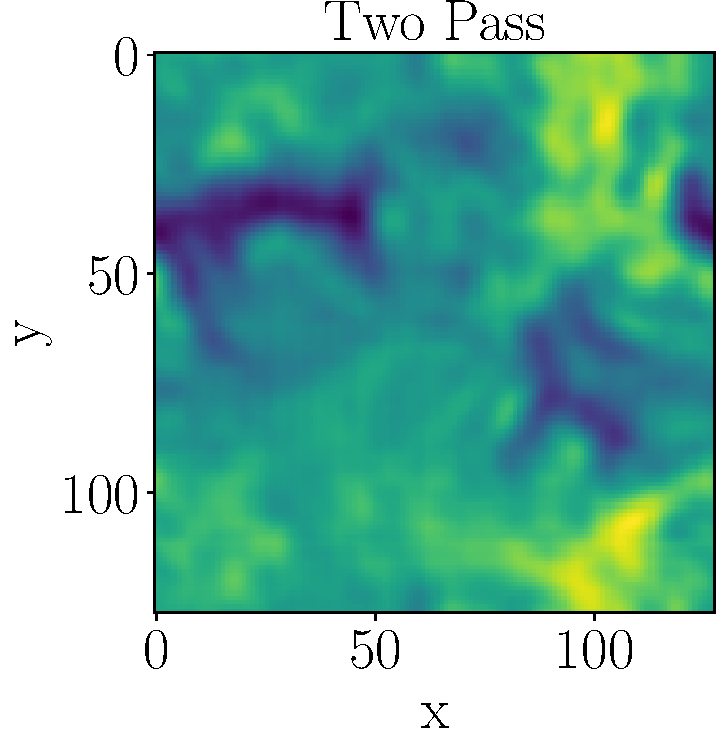
\includegraphics[height=3cm]{figure/T100_2pass.pdf}
	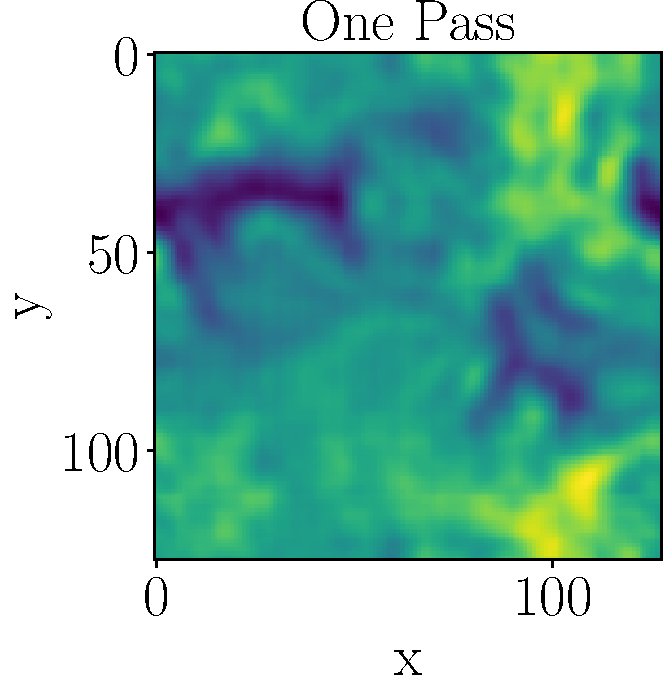
\includegraphics[height=3cm]{figure/T100_1pass.pdf}
	\centering
	\caption{\label{fig:T100}\textit{Visualizing Combustion Simulation:}
	All four figures show a slice of the temperature data along the first dimension.
	The approximation uses
	$\mathbf{r} = (281,25,25)$,
	$\mathbf{k} = (562,50,50)$,
	$\mathbf{s} = (1125, 101, 101)$,
	with the Gaussian TRP in the Tucker sketch.}
\end{figure}

\subsubsection{A second pass reduces error}
The second experiment compares our two-pass and one-pass algorithm.
The design is similar to the first experiment.
\ref{fig:vary-k-600-compare} shows that the two-pass algorithm
typically outperforms the one-pass algorithm,
especially in the high-noise, sparse, or rank-decay case.
Both converge at the same asymptotic rate.
(Results for other input tensors are available
\ifdefined \issupplement
in the supplement.)
\else
%in \ref{fig:vary-k-400-compare-app} and \ref{fig:vary-k-200-compare-app}
in \ref{appendix:more_result}.)
\fi

\subsubsection{Improvement on state-of-the-art}
The third experiment compares the performance of our two-pass and one-pass algorithms
and Tucker TensorSketch (T.--TS), as described in \cite{malik2018low},
the only extant one-pass algorithm.
For a fair comparison, we allocate the same storage budget to each algorithm
and compare the relative error of the resulting fixed-rank approximations.
We approximate synthetic 3D tensors with side length $I = 300$
with Tucker rank $r = 10$.
We use the suggested parameter settings for each algorithm:
$k = 2r$ and $s =2k+1$ for our methods; $K = 10$ for T.--TS.
Our one-pass algorithm
(with the Gaussian TRP)
uses $((2k+1)^N + kIN)$ storage,
whereas T.-TS uses $(Kr^{2N}+Kr^{2N-2})$ storage
\ifdefined \issupplement
(see supplement).
\else
(see \ref{tab:storage-comparison} in \ref{appendix: time-complexity}).
\fi

% Specifically, we choose $k$ linear in log scale within $\in [12,115]$,
% corresponding to $K \in [0.026,12]$ in \cite{malik2018low} \ref{fig:vary-memory}.

Figure \ref{fig:vary-memory} shows that our algorithms generally perform as well as T.--TS,
and dramatically outperforms for small storage budgets.
%two-pass algorithm always outperforms our one-pass algorithm, by a modest margin.
For example, our method achieves 1/50, 1/50, 1/7, and 1/4 the relative error of T.--TS
for low rank and sparse low rank ($\gamma = 0.01$), low rank ($\gamma = 0.1$), and polynomial-decay
input tensors, respectively.
For the low rank ($\gamma = 1$) tensor, the performance of T.--TS is not even monotone as the storage budget increases!
% In the case when the design tensor has a rank decay along its super diagonal, our algorithm is able to easily recover the low-rank signal, while their method is highly unstable and likely to give a worse result even in their suggested setting.
The performance of T.--TS is comparable with that of
the algorithms presented in this paper only when the storage budget is large.
%In both the low-rank and sparse low-rank settings, their method outperforms our method for very large memory usage.

\begin{remark}
	The paper \cite{malik2018low} proposes a multi-pass method, Tucker Tensor-Times-Matrix-TensorSketch (TTMTS) that is dominated by the one-pass method Tucker TensorSketch(TS) in all numerical experiments;
  hence we compare only with T.-TS.
\end{remark}

\subsection{Applications}\label{s-real-data}

We also apply our method to datasets drawn from three application domains:
climate, combustion, and video.
\begin{itemize}
\item \emph{Climate data.}
We consider global climate simulation datasets from
the Community Earth System Model (CESM) Community Atmosphere Model (CAM) 5.0 \cite{hurrell2013community,kay2015community}.
The dataset on aerosol absorption has four dimensions:
times, altitudes, longitudes, and latitudes  ($240 \times 30 \times 192 \times 288$).
% show in appendix
The data on net radiative flux at surface and dust aerosol burden have three dimensions:
times, longitudes, and latitudes ($1200 \times 192 \times 288$).
Each of these quantitives has a strong impact on the absorption of solar radiation and on cloud formation.

\item \emph{Combustion data.}
We consider combustion simulation data from \cite{lapointe2015differential}.
% This paper aims to understand the effect of differential diffusion, distributed burning,
% and local distinction under different circumstances.
The data consists of three measured quantities ---
pressure, CO concentration, and temperature ---
each observed on a $1408 \times 128 \times 128$ spatial grid.
% At each time, we choose three measured quantities out of the 40 measured quantities (all of size $1408 \times 128 \times 128$) at different locations to compress, specifically the pressure, CO concentration, and temperature.

\item \emph{Video data.}
We use our streaming method to cluster frames of a video,
as in \cite{malik2018low}.
Here, a low frame rate camera is mounted in a fixed position as people walk by.
A 3D tensor is constructed with each video frames as a slice.
%The rank of the tensor corresponds to the number of people seen. (The background is rank 2.)
The video consists of 2493 frames, each of size 1080 by 1980.
%  in grayscale,
% thus of size (2493 $\times$ 1080 $\times$ 1980).
As a tensor, stored as a \texttt{numpy.array}, the video data is 41.4 GB in total.
\end{itemize}

\subsubsection{Data compression}
We show that our proposed algorithms are able to
successfully compress climate and combustion data
even when the full data does not fit in memory.
%, we want to compress the huge original tensor into a low-rank Tucker decomposition efficiently.
Since the Tucker rank of the original tensor is unknown, we perform experiments for
three different target ranks. In this experiment, we hope to understand the effect of different choices of storage budget $k$ to
 achieve the same compression ratio. We define the compression ratio
 as the ratio in size between the original input tensor and the output Tucker factors, i.e. $\frac{\prod_{i = 1}^N I_i}{\sum_{i=1}^Nr_iI_i+ \prod_{i = 1}^N r_i}$.
As in our experiments on simulated data, \ref{fig:climate} shows
that the two-pass algorithm outperforms the one-pass algorithm as expected.
However, as the storage budget $k$ increases, both methods converge to the performance of HOOI.
The rate of convergence is faster for smaller target ranks.
Performance of our algorithms on the combustion simulation is qualitatively similar,
but converges faster to the performance of HOOI. \ref{fig:T100} visualizes the recovery of
the temperature data in combustion simulation for a slice along the first dimension. We could observe that the
recovery for both two-pass and one-pass algorithm approximate the recovery from HOOI.
% Indeed, but in general with a faster convergence rate than the climate data even when the data is not perfectly low rank, like the pressure data.
\ifdefined \issupplement
Similar results on other datasets appear in the supplement.)
\else
\ref{fig:srfrad_burden_dust} in \ref{appendix:more_real_data_result}
shows similar results on another dataset.
\fi

\subsubsection{Video scene classification}
We show how to use our single pass method to classify scenes in the video data described above.
The goal is to identify frames in which people appear.
% In our experiment, we split the dataset into nine segments each of size $277 \times 1080 \times 1980$.
% \mnote{why split?}
We remove the first 100 frames and last 193 frames where the camera setup happened,
as in \cite{malik2018low}.
We stream over the tensor and sketch it using parameters $k = 300, s = 601$.
Finally, we compute a fixed-rank approximation with $\mathbf{r} = (10,10,10)$ and $(20,20,20)$.
We apply K-means clustering to the resulting 10 or 20 dimensional vectors
corresponding to each of the remaining 2200 frames.

We experimented with clustering vectors found in three ways:
from the two-pass or one-pass Tucker approximation,
or directly from the factor sketch. % without performing the reconstruction.

When matching the video frames with the classification result,
we can see that the background light is relatively dark at the beginning,
thus classified into \texttt{Class} $0$.
After a change in the backgroun light,
most other frames of the video are classified into \texttt{Class} $1$.
When a person passes by the camera, the frames are classified into \texttt{Class} $2$.
Right after the person passed by, the frames are classified into \texttt{Class} $0$,
the brighter background scene, due to the light adjustment.

Our classification results (using the linear sketch or approximation)
are similar to those in \cite{malik2018low}
while using only $1/500$ as much storage; the one pass approximation
requires more storage (but still less than \cite{malik2018low}) 
to achieve similar performance.
In particular, using the sketch itself, rather than the Tucker approximation,
to summarize the data enables very efficient video scene classification.

On the other hand, to reconstruct the original video frames
we require much larger $\mathbf{k}$ and $\mathbf{r}$:
the video is not very low rank along the spatial dimensions.
\ref{fig:Frame500} shows that
even with $\mathbf{s} = {601, 601, 601}, \mathbf{k} = (300, 300, 300), \mathbf{r} = (50, 50, 50)$, the recovered frame is very noisy.
% The memory and computational requirements of HOOI exceed our capacity,
% so we cannot apply it to the video data.
